\section{Introduction}

Evolutionary algorithms are classified as meta-heuristic search algorithms, where possible solution elements span the n-dimensional search space to find the global optimum solution. Over the years, natural phenomena and biological processes have laid the foundation for several algorithms for control and optimization that have highlighted their applicability in solving intricate optimization problems in various fields.At the cellular level in the E.Coli Bacterium,there is sensing and locomotion involved in seeking nourishment and avoid harmful chemicals.These behavioral characterisitics have fueled the inspiration for the bacterial foraging optimization algorithm. Ant Colony Optimization(ACO) deals with behaviour of ants and has been a successful model for solving complex problems. PSO is a swarm intelligence algorithm based on behaviour of birds anf fishes that models these particles as they traverse an n-Dimensional search space and share information in order to obtain global optimum.
From a biological control point, the human brain represents one of the most sophesticated architectures and several research attempts seek to mimic its accuracy, precision and efficiency.The brain function activities can be classified into 2 categories:- sensory and motor operations. Sensory cortical functions inspired concept of neural networks and they are being scaled successfully in deep learning to solve vast amount of problems. 
The human motor function represents a neural distributed and hierarchical control system. It can be classified as having local control functions for movement as well as higher level controllers for gross motion and decision making for planning actions.The optimal execution of motor operation involves distributed brain structures at different levels of hierarchy.These include the pre-frontal cortex, motor cortex, spinal cord, anterior horn cells etc. For generating an actions sequence, a sequence of actions is implemented by a string of subsequences of actions each implemented in a different part of the body. The operational structure has been depicted in Figure 1.[]
For optimality of actions, neurons act in unison. The neurons in the motor cortex act like global leaders and send inhibitory or facilitatory influence over the anterior horn cells, local leaders, located in the spinal cord. These local leaders, are connected to the muscle fibres, effectors through a peripheral nerve and neuromuscular junction.
Efficient execution of task requires feedback based facilitation and inhibition of the effectors over the anterior horn cells. These sequence of operations consitute the optimal convergence of the system leading to smooth motor execution.

The present paper focusses on introducing an optimisation algorithm modelled intuitively on the distributed and hierarchical operation of the brain motor function. We seek to exploit the <> inherent structure of the popular Differential Evolution algorithm by extrapolating the <Add a Line>. The algorithm performance is exhaustively compared on the <Add here and connect to different algorithms>.<Why we have extrapolated DE>.<How introducing Hierarchy has ensured faster convergence and better optimization that other adaptive variants that have been discussed like JADE>.

Lorem ipsum dolor sit amet, consectetur adipiscing elit, sed do eiusmod tempor incididunt ut labore et dolore magna aliqua. Ut enim ad minim veniam, quis nostrud exercitation ullamco laboris nisi ut aliquip ex ea commodo consequat. Duis aute irure dolor in reprehenderit in voluptate velit esse cillum dolore eu fugiat nulla pariatur. Excepteur sint occaecat cupidatat non proident, sunt in culpa qui officia deserunt mollit anim id est laborum.Lorem ipsum dolor sit amet, consectetur adipiscing elit, sed do eiusmod tempor incididunt ut labore et dolore magna aliqua. Ut enim ad minim veniam, quis nostrud exercitation ullamco laboris nisi ut aliquip ex ea commodo consequat. Duis aute irure dolor in reprehenderit in voluptate velit esse cillum dolore eu fugiat nulla pariatur. Excepteur sint occaecat cupidatat non proident, sunt in culpa qui officia deserunt mollit anim id est laborum.


% Operational maturity of biological control systems have enamored researchers across various domains.Consequently, these have been the source of inspiration of various mathematical and logical models for control, automation and optimization. The behavioural characteristics observed at the Cellular level in E.Coli fueled the inspiration for the Bacterial Foraging Optimization algorithm.

% The biological system most relevant to us is the human brain. It represents the most advanced control architecture and several research initiative seek to mimic its level of accuracy and precision in day-to-day activities. The brain activities can be distributed into two categories: sensory and motor operations. Sensory cortical functions have to an extent inspired the concept of neural networks that have been successfully scaled to a large number of domains. 

% While not always the case, it is at times useful and accurate to view a biological neural network as being arranged in a hierarchical fashion. As a naive example, consider a day-to-day activity of grasping a cup of coffee.
% One part of the brain that is clearly hierarchical is the human motor system. The hierarchical and distributed control of the human motor system can be classified as having local control functions for movement and higher level controllers that facilitate gross motion and decision making.

% The optimal execution of any human motor operation, such as grasping a cup of coffee, involves distributed brain structures at different levels of hierarchy. It broadly includes the prefrontal cortex, motor cortex, spinal cord, anterior horn cells etc. In generating actions sequences, a sequence of actions is implemented by string of subsequences of actions, each possibly implemented in different parts of the body.

% The hierarchy of the operations can be classified as:

% \begin{itemize}
% \item[1.] Motivation and planning of the movement or task.
% \item[2.] Generation of instructions for movement.
% \item[3.] Refinement of instruction based on feedback from components.
% \item[4.] Maintenance of posture and smooth execution of task.
% \end{itemize}

% Whenever a person plans to perform an action, electrical signal generated from the pyramidal neurons in the prefrontal cortex(global leaders, center for the decision making) are transmitted a supraspinal tract on the anterior horn cells(communicating to local leaders). Initially, these global leaders send inhibitory influence to the population over the local leaders. Efficient and optimal execution of tasks involves feedback based facilitation and inhibition of the effectors. These result in contraction and relaxation of the agonist and antagonist muscle fibers through the local leaders. The sequence of updation of the represents the optimal convergence of the system, leading to smooth motor operations.

\section{Classical Differential Evolution}

The classical Differential Evolution (DE) algorithm is a population-based global optimization algorithm, utilizing a crossover and mmutation approach to generate new individuals in the population for achieving optimum solutions. For each individual $x_i$ that belongs to the population, DE randomly samples three other individuals from the population $a_i$, $b_i$ and $c_i$. Then using the randomly chosen points, a new individual vector is generated using equation \eqref{de}:

\begin{equation}
\label{de}
u_i = a_i + F (b_i - c_i)
\end{equation}

Where, $F$ is called the differential weight (Usually lies between $[0, 1]$).\\
And to obtain the new position of the individual, a crossover operation is implemented between $x_i$ and $u_i$, controlled by the parameter $CR$ called the crossover probability. The value for $CR$ always lies between $[0, 1]$.

\begin{figure}[h!]
  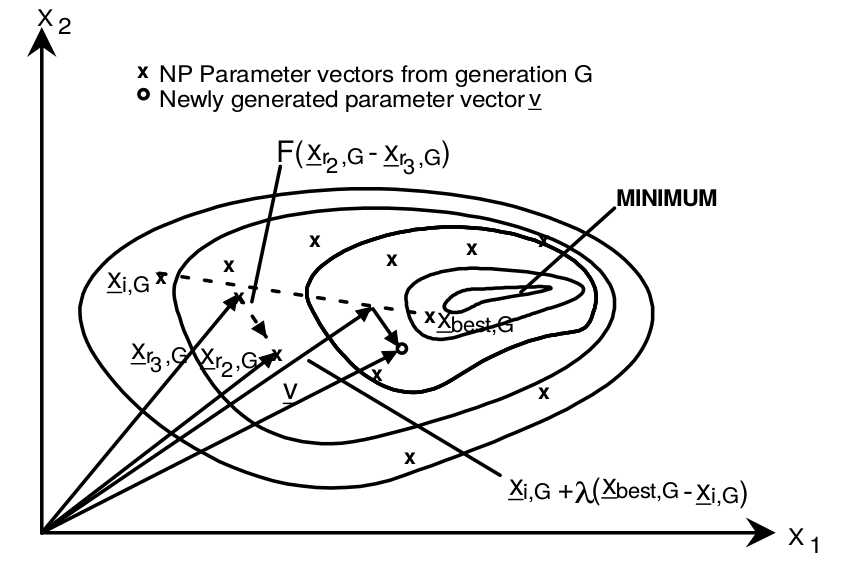
\includegraphics[scale=0.3]{contourDE}
  \caption{Two dimensional example of an objective function showing its contour lines and the process for
generating v in scheme DE2}
  \label{fig:contourDE}
\end{figure}

\begin{figure}[h!]
  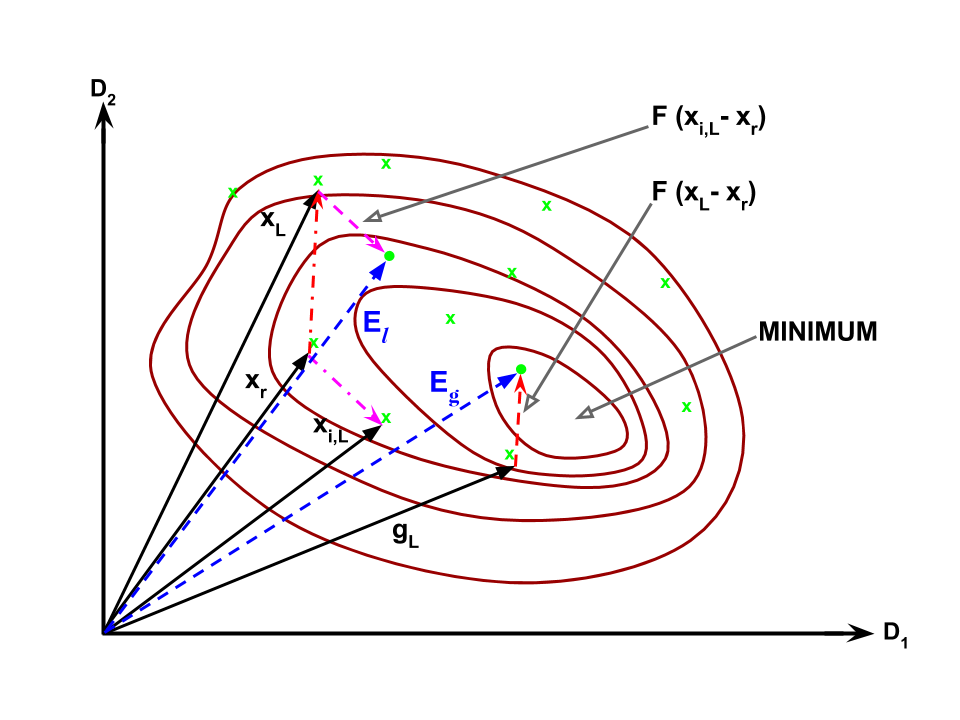
\includegraphics[scale=0.25]{contourDL}
  \caption{The process for generating generation of $E_g$ and $E_l$ in a 2 dimensional optimization.}
  \label{fig:contourDL}
\end{figure}
%%%%%%%%%%%%%%%%%%%%%%%%%%%%%%%%%%%%%%%%%%%%%%%%%%%%%%%%%%%%%%%%%%%%%%%%%%%%%%%%%%%%%%%%%%%%%%%%%%%%%%%%%%%%%%

\section{Distributed Leader Optimization}

Taking inspiration from the human motor system, we model the hierarchical motor operations in our optimization agents, where we define a global leader which influences the action of several distributed local leaders and the particle agents which act as the effectors. The global leader is analogous to the decision making and planning section in the motor system hierarchy whilst, the local leaders correspond to motion generators acting under the influence of the  global leader.

The position of each particle in the population is affected by the influence of global leaders and local leaders, while also being affected by a randomly chosen particle from the population to induce some stochasticity in the optimization pipeline. We first model the influence of the global leader on the local leaders and the influences of the local leaders  on each population element using equation \eqref{one} and \eqref{two}. We introduce a hierarchical crossover between the two influencing equations governed by a hierarchical crossover parameter $HC$.

\begin{algorithm}
\caption{Distributed Leader Optimization}
\label{algo}
\begin{algorithmic}[1]
  \Procedure{Start}{}
    \State Initialize parameters ($HC$, $P$, $N_l$, $N$).
    \State Generate initial global leader $g_L$ as a random point.
    \State Generate $N_l$ local leader points around $g_L$.
    \State Using a Normal distribution, generate $N$ points for population $P$ around the local leaders.
    \While{termination criteria is not met}
    %%%%%%%%%%%%%%%%%%%%%%%%%%%%%%%%%%%%%%%%%%%%%%%%%%%%%%%%%%%%%%%%%%%%%%%%%%%%%%%%%%%%%%
      \For{each individual $x_i$ in $P$}
        \State compute the corresponding local leader $l$ based on nearest position.
        \State Let $u = 0$ be an empty vector.
        \State Let $i_c$ and $i_N$ be the current generation and total generations of the procedure.
        \If {$i_c \textless (HC*i_N)$}
          \State $u = E_g$ from \eqref{one}.
        \Else
          \State $u = E_l$ from \eqref{two}.
        \EndIf
        
        \For{each dimension $i$}
          \State Generate $r_i = U(0, 1)$, a random number between 0 and 1.
          \If {$r_i \textless HC$}
            \State Set $x_i^{'} = x_i$.
          \Else
            \State Set $x_i^{'} = u_i$
          \EndIf
        \EndFor
        \If {$f(x^{'}) \textless f(x)$}
          \State Replace $x$ with $x^{'}$ in the population.
        \EndIf
      \EndFor
      \State Alter local leaders in each population cluster based on objective function value.
      \State Compute updated global leader $g_L$.
    \EndWhile
  \EndProcedure
\end{algorithmic}
\end{algorithm}

Analogously to [step 3] in the brain motor operation, the updation of particle positions requires generating feedback for the leaders as a part of the optimization procedure, and hence the local leaders and the global leader are updated based onn their objective function value generated from the perturbations in population particles. This series of events comprise of one optimization pass (one loop step). On execution of several optimization passes as described, the system is able to converge to an optimal configuration, analogous to the successful execution of the required task as shown in [step 4].

The updated position of the particle $x$ is governed by the hierarchical crossover operation and a mutation operation. The hierarchical operation is affected by the global leader $g_L$ and the local leader $l$ through the parametric equations \eqref{one} and \eqref{two}. Switching between the two is governed by the hierarchical crossover parameter $HC$. The given equations are discussed as follows:

\begin{equation}
\label{one}
E_g = g_L + F (l - c)
\end{equation}

\begin{equation}
\label{two}
E_l = l + F (x - c)
\end{equation}



In the algorithm \ref{algo}, The Hierarchical crossover is controlled by the conditional equation $i_c \textless (HC*i_N)$. According to this equation, during the initial phases ($HC$ fraction of total generations) of the optimization procedure, only the local leader is responsible for the motion of the agents, and after a certain amount of time has passed, the global leader also takes part in the motion generation process, signifying the motor control operation.
Additionaly, The hierarchical crossover parameter $HC$ also influences the mutation process wherein the degree of final mutation is decided based on the probability $HC$.

%%%%%%%%%%%%%%%%%%%%%%%%%%%%%%%%%%%%%%%%%%%%%%%%%%%%%%%%%%%%%%%%%%%%%%%%%%%%%%%%%%%%%%%%%%%%%%%%%%%%%%%%%%%%%%
\section{Results and Discussions}

All evaluations were performed using Python 2.7.12 with Scipy and Numpy for numerical computations and Matplotlib package for graphical representation of the result data. This section is divided into two sub-sections: Section A provides description about the problem set used for analysis of algorithmic efficiency and accuracy, and section B comprises of tabular and graphical data to support the claim of eminence of the proposed approach.

\subsection{Problem Set Description}

The set of objective functions considered for testing the proposed algorithm and compare it's performance against DE, Particle Swarm Optimization Differential Evolution (PSODE) and Joint Adaptive Differential Evolution (JADE) has been taken from the CEC 2017 [] set of benchmark functions.

\begin{table}[!htbp]
\caption{CEC 2017 Test Functions}
\centering
%\def\arraystretch{2.0}
\begin{tabular}{|p{0.5cm}|p{5.4cm}|p{0.6cm}|}
\hline
F$_{id}$ & Problem Function & F* \\ \hline
$f_{1}$ & Shifted and Rotated Bent Cigar Function & 100 \\
\hline
$f_{2}$ & Shifted and Rotated Sum of Different Power Function & 200 \\
\hline
$f_{3}$ & Shifted and Rotated Zakharov Function & 300\\
\hline
$f_{4}$ & Shifted and Rotated Rosenbrock's Function & 400\\
\hline
$f_{5}$ & Shifted and Rotated Rastrigin's Function & 500\\
\hline
$f_{6}$ & Shifted and Rotated Expanded Scaffer's F6 Function & 600\\
\hline
$f_{7}$ & Shifted and Rotated Lunacek Bi\_Rastrigin Function & 700\\
\hline
$f_{8}$ & Shifted and Rotated Non-Continuous Rastrigin's Function & 800\\
\hline
$f_{9}$ & Shifted and Rotated Levy Function & 900\\
\hline
$f_{10}$ & Shifted and Rotated Schwefel's Function & 1000\\
\hline
$f_{11}$ & Hybrid Function 1 (N=3) & 1100\\
\hline
$f_{12}$ & Hybrid Function 2 (N=3) & 1200\\
\hline
$f_{13}$ & Hybrid Function 3 (N=3) & 1300\\
\hline
$f_{14}$ & Hybrid Function 4 (N=4) & 1400\\
\hline
$f_{15}$ & Hybrid Function 5 (N=4) & 1500\\
\hline
$f_{16}$ & Hybrid Function 6 (N=4) & 1600\\
\hline
$f_{17}$ & Hybrid Function 7 (N=5) & 1700\\
\hline
$f_{18}$ & Hybrid Function 8 (N=5) & 1800\\
\hline
$f_{19}$ & Hybrid Function 9 (N=5) & 1900\\
\hline
$f_{20}$ & Hybrid Function 10 (N=6) & 2000\\
\hline
$f_{21}$ & Composition Function 1 (N=3) & 2100\\
\hline
$f_{22}$ & Composition Function 2 (N=3) & 2200\\
\hline
$f_{23}$ & Composition Function 3 (N=4) & 2300\\
\hline
$f_{24}$ & Composition Function 4 (N=4) & 2400\\
\hline
$f_{25}$ & Composition Function 5 (N=5) & 2500\\
\hline
$f_{26}$ & Composition Function 6 (N=5) & 2600\\
\hline
$f_{27}$ & Composition Function 7 (N=6) & 2700\\
\hline
$f_{28}$ & Composition Function 8 (N=6) & 2800 \\
\hline
$f_{29}$ & Composition Function 9 (N=3) & 2900 \\
\hline
$f_{30}$ & Composition Function 10 (N=3) & 3000 \\
\hline
\multicolumn{3}{|c|}{ } \\[0.05ex]
\multicolumn{3}{|c|}{Search Range: [-100,100]$^{D}$ } \\
\hline
\end{tabular}
\vspace{-1mm}
\end{table}



\subsection{Results}

\begingroup
\renewcommand\arraystretch{0.7}
\begin{table*}[t!]
\centering
\caption{Objective Function Value for Dimension: 10}
\vspace{-3mm}
 \begin{tabular}{|p{0.8cm}|p{1.6cm}|p{1.6cm}|p{1.6cm}|p{1.6cm}|p{1.6cm}|p{1.6cm}|p{1.6cm}|p{1.6cm}|} 
 \hline
 ID & \multicolumn{2}{c|}{DE} & \multicolumn{2}{c|}{JADE} & \multicolumn{2}{c|}{PSODE} & \multicolumn{2}{c|}{HIDE} \\
 \hline
    & best & mean & best & mean & best & mean & best & mean \\ [0.5ex] 
 \hline
$f_1$  & 100.000051 & 100.011085 & \textbf{100.0} & \textbf{100.0} & 100.000712 & 185.975885 & \textbf{100.0} & \textbf{100.0} \\ 
 % \hline
$f_2$  & \textbf{200.0} & 200.1 & \textbf{200.0} & \textbf{200.0} & \textbf{200.0} & \textbf{200.0} & \textbf{200.0} & \textbf{200.0} \\ 
 % \hline
$f_3$  & 300.00134 & 300.214502 & \textbf{300.0} & \textbf{300.0} & 300.000006 & 300.000985 & \textbf{300.0} & \textbf{300.0} \\ 
 % \hline
$f_4$  & 400.042617 & 403.674837 & \textbf{400.0} & 400.409399 & 400.064644 & 404.307763 & \textbf{400.0} & \textbf{400.000003} \\ 
 % \hline
$f_5$  & 566.661791 & 604.867489 & \textbf{523.908977} & \textbf{541.521084} & 525.868824 & 575.61616 & 533.803201 & 579.483815 \\ 
 % \hline
$f_6$  & 621.914237 & 634.807962 & 620.878276 & 636.034759 & \textbf{603.187964} & 635.865001 & 613.730565 & \textbf{629.293758} \\ 
 % \hline
$f_7$  & 724.831278 & 739.129935 & \textbf{717.016542} & \textbf{723.983312} & 725.44788 & 733.15638 & 720.345706 & 725.233785 \\ 
 % \hline
$f_8$  & \textbf{818.904202} & 829.749207 & 821.914433 & \textbf{826.321588} & 820.8941 & 830.246691 & 821.064763 & 828.160987 \\ 
 % \hline
$f_9$  & \textbf{900.0} & 908.104383 & \textbf{900.0} & 1084.478253 & \textbf{900.0} & 1124.102561 & \textbf{900.0} & \textbf{903.454324} \\ 
 % \hline
$f_{10}$  & 1911.510092 & 2447.443751 & 1760.956867 & 2162.648588 & 2049.644727 & 2518.241095 & \textbf{1694.437597} & \textbf{2049.074266} \\ 
 % \hline
$f_{11}$  & 1102.985708 & 1113.423105 & 1105.661676 & 1117.509748 & 1105.97013 & 1120.192974 & \textbf{1101.769749} & \textbf{1108.863598} \\ 
 % \hline
$f_{12}$  & 2531.746305 & 6509.743078 & 1438.605713 & 5430.674683 & 4089.006352 & 10810.387667 & \textbf{1308.438341} & \textbf{1327.405881} \\ 
 % \hline
$f_{13}$ & 1313.130226 & 1404.903601 & \textbf{1304.681558} & \textbf{1328.755262} & 1319.839199 & 1453.340785 & 1306.682039 & 1344.282241 \\ 
 % \hline
$f_{14}$  & 1409.949612 & 1426.571937 & 1412.934432 & 1428.169439 & 1420.91065 & 1434.112884 & \textbf{1404.928993} & \textbf{1410.000769} \\ 
 % \hline
$f_{15}$  & 1504.131392 & 1521.446614 & 1502.496189 & 1508.31154 & 1501.389515 & 1518.310358 & \textbf{1500.08137} & \textbf{1503.169264} \\ 
 % \hline
$f_{16}$  & 1958.42062 & 2104.555728 & 1958.857997 & 2094.630816 & \textbf{1958.411527} & \textbf{2048.156879} & 1958.433511 & 2062.385949 \\ 
 % \hline
$f_{17}$  & 1728.194973 & \textbf{1743.155244} & 1730.715318 & 1748.129878 & 1727.80039 & 1791.607742 & \textbf{1723.853972} & 1747.589077 \\ 
 % \hline
$f_{18}$  & 1801.586012 & 1838.840555 & 1804.298538 & 1825.091639 & 1817.154641 & 1840.546923 & \textbf{1800.235516} & \textbf{1804.014301} \\ 
 % \hline
$f_{19}$  & 1901.195482 & 1903.604767 & 1900.399786 & 1902.152965 & 1902.71174 & 1906.252333 & \textbf{1900.005632} & \textbf{1901.014116} \\ 
 % \hline
$f_{20}$  & 2204.55412 & 2289.226577 & 2148.538938 & 2178.313173 & 2140.561308 & 2261.038768 & \textbf{2139.915527} & \textbf{2172.816519} \\ 
 % \hline
$f_{21}$  & 2337.772994 & 2387.230357 & \textbf{2314.421135} & \textbf{2338.688719} & 2337.207339 & 2351.898856 & 2320.496212 & 2344.61612 \\ 
 % \hline
$f_{22}$  & 2300.805852 & 2304.132879 & \textbf{2300.0} & \textbf{2300.093485} & 2300.684181 & 2301.710478 & 2300.000015 & 2301.095975 \\ 
 % \hline
$f_{23}$  & 3070.177083 & 3145.772296 & 3003.678563 & 3091.22041 & \textbf{2773.372859} & 3060.022519 & 2867.020036 & \textbf{3047.982305} \\ 
 % \hline
$f_{24}$  & \textbf{2500.0} & \textbf{2500.0} & \textbf{2500.0} & \textbf{2500.0} & \textbf{2500.0} & \textbf{2500.0} & \textbf{2500.0} & \textbf{2500.0} \\ 
 % \hline
$f_{25}$  & 2899.584968 & 2933.249812 & 2899.584968 & 2930.266506 & \textbf{2897.742869} & \textbf{2921.27479} & 2897.833388 & 2927.976511 \\ 
 % \hline
$f_{26}$  & \textbf{2800.0} & 4117.597033 & \textbf{2800.0} & \textbf{2956.064173} & \textbf{2800.0} & 3367.60765 & \textbf{2800.0} & 3161.548079 \\ 
 % \hline
$f_{27}$  & 3113.157656 & 3358.806434 & 3072.439023 & 3178.509645 & 3078.873134 & 3240.501812 & \textbf{3071.203569} & \textbf{3107.268539} \\ 
% \hline
$f_{28}$  & 3184.75565 & 3230.921422 & 3184.75565 & \textbf{3195.113042} & 3184.755652 & 3198.370691 & \textbf{3100.0} & 3195.411961 \\ 
 % \hline
$f_{29}$  & \textbf{3148.587115} & 3266.979786 & 3172.400194 & \textbf{3233.707677} & 3191.348193 & 3244.892638 & 3189.211417 & 3292.420474 \\ 
 % \hline
$f_{30}$  & 3442.555095 & 11927.404685 & 3207.766942 & 4615.591316 & 4573.358512 & 16415.162901 & \textbf{3205.740954} & \textbf{3249.710975} \\
\hline
$w/t/l$  & 2/4/24 & 1/1/28 & 5/7/18 & 9/4/17 & 4/4/22 & 2/2/26 & 12/7/11 & 14/4/12 \\
\hline

\end{tabular}
\end{table*}

\begin{table*}[t!]
\centering
\caption{Objective Function Value for Dimension: 30}
\vspace{-3mm}
 \begin{tabular}{|p{0.8cm}|p{1.6cm}|p{1.6cm}|p{1.6cm}|p{1.6cm}|p{1.6cm}|p{1.6cm}|p{1.6cm}|p{1.6cm}|} 
 \hline
$f_{id}$ & \multicolumn{2}{c|}{DE} & \multicolumn{2}{c|}{JADE} & \multicolumn{2}{c|}{PSODE} & \multicolumn{2}{c|}{HIDE} \\
 \hline
    & best & mean & best & mean & best & mean & best & mean \\ [0.5ex] 
 \hline
$f_{1}$ & 100.001508 & 4334.438478 & 100.001338 & 100.056201 & 364.295574 & 4236.363207 & \textbf{100.0} & \textbf{100.0} \\ 
 % \hline
$f_{2}$  & 40412441.0 & 5.129601e+19 & \textbf{200.0} & 1535352368.6 & 332899.0 & 9.590679e+11 & \textbf{200.0} & \textbf{159855.5} \\ 
 % \hline
$f_{3}$  & 17926.872873 & 22131.542719 & 69304.926091 & 74080.700372 & 15792.547575 & 21683.209092 & \textbf{3679.811599} & \textbf{8999.947269} \\ 
 % \hline
$f_{4}$  & 481.255055 & 519.422652 & 403.633939 & \textbf{442.206911} & 468.341175 & 479.341966 & \textbf{400.004163} & 443.016156 \\ 
 % \hline
$f_{5}$  & 689.041352 & 737.79326 & \textbf{667.50756} & \textbf{735.204027} & 715.904429 & 746.548906 & 685.40454 & 738.842184 \\ 
 % \hline
$f_{6}$  & \textbf{643.626307} & 652.582714 & 651.39169 & 655.142819 & 642.724237 & 655.106996 & 644.701241 & \textbf{652.002395} \\ 
 % \hline
$f_{7}$  & 883.347367 & 962.591129 & \textbf{779.907693} & \textbf{818.344111} & 790.014281 & 854.285524 & 812.923573 & 856.90477 \\ 
 % \hline
$f_{8}$  & 923.37426 & 967.251501 & 931.500175 & \textbf{957.362003} & \textbf{915.414882} & 960.486239 & 930.288539 & 964.11663 \\ 
 % \hline
$f_{9}$  & 5652.483961 & 7878.781444 & 4953.05469 & 5146.600953 & 6018.417197 & 9042.410178 & \textbf{4003.118072} & \textbf{4734.984364} \\ 
 % \hline
$f_{10}$  & \textbf{3596.63104} & 4536.989761 & 4012.723292 & \textbf{4204.18969} & 3934.606704 & 4863.741107 & 3793.781776 & 4346.741344 \\ 
 % \hline
$f_{11}$  & 1162.405965 & 1184.634006 & 1152.748529 & 1174.58813 & 1165.144993 & 1189.171787 & \textbf{1149.748499} & \textbf{1171.130409} \\ 
 % \hline
$f_{12}$  & 56679.435092 & 317650.61349 & 24821.171765 & 58930.090242 & 10221.077465 & 161046.05540 & \textbf{9208.289246} & \textbf{41947.22269} \\ 
 % \hline
$f_{13}$  & 3002.029489 & 18794.835991 & 4276.907742 & 13775.816239 & 3871.279833 & 10612.26359 & \textbf{1664.06241} & \textbf{2453.606969} \\ 
 % \hline
$f_{14}$  & 1773.180798 & 5502.160382 & 1496.219858 & 42868.9158 & 1555.452763 & 4029.808535 & \textbf{1462.926848} & \textbf{1504.191515} \\ 
 % \hline
$f_{15}$  & 1860.435669 & 2484.689969 & 1688.05046 & 2222.674323 & 1651.747476 & 2223.060542 & \textbf{1611.074402} & \textbf{1852.66177} \\ 
 % \hline
$f_{16}$  & 2517.439623 & 2827.004968 & 2344.19818 & 2621.618684 & \textbf{2239.242719} & \textbf{2664.114667} & 2298.041965 & 2691.674809 \\ 
 % \hline
$f_{17}$  & 2321.175936 & 2604.529778 & 2062.898023 & 2546.995596 & 2107.43677 & 2457.34021 & \textbf{1820.806639} & \textbf{2418.723829} \\ 
 % \hline
$f_{18}$  & 38987.282456 & 94156.328505 & \textbf{11841.60813} & 184888.162181 & 62294.853257 & 118430.28912 & 12578.003784 & \textbf{23024.11193} \\ 
 % \hline
$f_{19}$  & 2043.469888 & 3010.235379 & 1959.71819 & 2156.957875 & 3049.52231 & 6840.408394 & \textbf{1949.271714} & \textbf{1987.866761} \\ 
 % \hline
$f_{20}$  & 2625.539158 & 2864.832611 & \textbf{2706.314441} & \textbf{2805.600064} & 2619.996493 & 2895.107238 & 2753.806213 & 2966.035793 \\ 
 % \hline
$f_{21}$  & 2412.081757 & 2504.777775 & 2414.52134 & 2456.718982 & 2431.740293 & 2478.841357 & \textbf{2200.0} & \textbf{2442.734316} \\ 
 % \hline
$f_{22}$  & 2300.481796 & 5655.569322 & \textbf{2300.0} & \textbf{4157.698784} & 2307.721358 & 6811.069162 & 2300.009985 & 6795.24842 \\ 
 % \hline
$f_{23}$  & 3050.654508 & 3572.965066 & \textbf{2772.002023} & \textbf{2946.749322} & 2764.922461 & 3199.874364 & 2883.276891 & 3543.839343 \\ 
 % \hline
$f_{24}$  & 3104.623692 & 3290.698756 & 2891.557648 & 2965.225566 & \textbf{2911.63347} & 2983.772932 & \textbf{2500.0} & 2940.75997 \\ 
 % \hline
$f_{25}$  & 2916.180657 & 2946.711753 & 2875.106846 & 2881.091389 & 2875.498843 & 2889.943671 & \textbf{2874.171109} & \textbf{2877.484904} \\ 
 % \hline
$f_{26}$  & 4043.691403 & 6756.3724 & 2900.0 & \textbf{3266.510982} & \textbf{2800.007809} & 3273.128769 & 2900.0 & 3298.490539 \\ 
 % \hline
$f_{27}$  & 3200.005857 & 3998.876498 & 3145.810354 & \textbf{3189.82261} & 3145.425231 & 3639.634132 & \textbf{3132.816283} & 3284.28897 \\ 
 % \hline
$f_{28}$  & 3290.744025 & 3326.263983 & \textbf{3100.0} & 3131.027315 & 3195.486838 & 3225.594053 & \textbf{3100.0} & \textbf{3115.505829} \\ 
 % \hline
$f_{29}$  & 3720.314598 & 4115.185803 & \textbf{3305.310139} & \textbf{3626.887552} & 3535.952295 & 3867.593068 & 3352.845055 & 3709.102375 \\ 
 % \hline
$f_{30}$  & 3359.030768 & 3900.826662 & \textbf{3263.496536} & 3749.610722 & 3312.635025 & 3524.714477 & 3298.704645 & \textbf{3421.715322} \\ 
\hline
$w/t/l$  & 2/0/28 & 0/0/30 & 8/2/20 & 11/0/19 & 4/0/26 & 1/0/29 & 15/2/13 & 17/0/13 \\
\hline
\end{tabular}
\end{table*}
\endgroup


%\begin{table*}[t!]
\centering
\caption{Objective Function Value for Dimension: 30}
\resizebox{1.6\columnwidth}{!}{
 \begin{tabular}{|p{0.8cm}|p{1.6cm}|p{1.6cm}|p{1.6cm}|p{1.6cm}|p{1.6cm}|p{1.6cm}|p{1.6cm}|p{1.6cm}|} 
 \hline
$f_{id}$ & \multicolumn{2}{c|}{DE} & \multicolumn{2}{c|}{JADE} & \multicolumn{2}{c|}{PSO-DE} & \multicolumn{2}{c|}{HIDE} \\
 \hline
    & best & mean & best & mean & best & mean & best & mean \\ [0.5ex] 
 \hline
$f_{1}$ & 100.001508 & 4334.43848 & 100.001338 & 100.056201 & 364.295574 & 4236.36321 & \textbf{100.0} & \textbf{100.0} \\ 
 % \hline
$f_{2}$  & 40412441.0 & 5.1296e+19 & \textbf{200.0} & 1535352368 & 332899.0 & 9.59068e+11 & \textbf{200.0} & \textbf{159855.5} \\ 
 % \hline
$f_{3}$  & 17926.8728 & 22131.5427 & 69304.9261 & 74080.7004 & 15792.5475 & 21683.2090 & \textbf{3679.81159} & \textbf{8999.94726} \\ 
 % \hline
$f_{4}$  & 481.255055 & 519.422652 & 403.633939 & \textbf{442.206911} & 468.341175 & 479.341966 & \textbf{400.004163} & 443.016156 \\ 
 % \hline
$f_{5}$  & 689.041352 & 737.79326 & \textbf{667.50756} & \textbf{735.204027} & 715.904429 & 746.548906 & 685.40454 & 738.842184 \\ 
 % \hline
$f_{6}$  & \textbf{643.626307} & 652.582714 & 651.39169 & 655.142819 & 642.724237 & 655.106996 & 644.701241 & \textbf{652.002395} \\ 
 % \hline
$f_{7}$  & 883.347367 & 962.591129 & \textbf{779.907693} & \textbf{818.344111} & 790.014281 & 854.285524 & 812.923573 & 856.90477 \\ 
 % \hline
$f_{8}$  & 923.37426 & 967.251501 & 931.500175 & \textbf{957.362003} & \textbf{915.414882} & 960.486239 & 930.288539 & 964.11663 \\ 
 % \hline
$f_{9}$  & 5652.48396 & 7878.78144 & 4953.05469 & 5146.60095 & 6018.41719 & 9042.41018 & \textbf{4003.11807} & \textbf{4734.98436} \\ 
 % \hline
$f_{10}$  & \textbf{3596.63104} & 4536.98976 & 4012.72329 & \textbf{4204.18969} & 3934.60671 & 4863.74111 & 3793.78177 & 4346.74134 \\ 
 % \hline
$f_{11}$  & 1162.40596 & 1184.63401 & 1152.74853 & 1174.58813 & 1165.14499 & 1189.17178 & \textbf{1149.74849} & \textbf{1171.13041} \\ 
 % \hline
$f_{12}$  & 56679.4351 & 317650.613 & 24821.1717 & 58930.0902 & 10221.0774 & 161046.055 & \textbf{9208.28924} & \textbf{41947.2226} \\ 
 % \hline
$f_{13}$  & 3002.02949 & 18794.8359 & 4276.90774 & 13775.8162 & 3871.27983 & 10612.2635 & \textbf{1664.06241} & \textbf{2453.60697} \\ 
 % \hline
$f_{14}$  & 1773.18079 & 5502.16038 & 1496.21986 & 42868.9158 & 1555.45276 & 4029.80853 & \textbf{1462.92685} & \textbf{1504.19151} \\ 
 % \hline
$f_{15}$  & 1860.43566 & 2484.68996 & 1688.05046 & 2222.67432 & 1651.74747 & 2223.06054 & \textbf{1611.07440} & \textbf{1852.66177} \\ 
 % \hline
$f_{16}$  & 2517.43962 & 2827.00496 & 2344.19818 & 2621.61868 & \textbf{2239.24272} & \textbf{2664.11466} & 2298.04196 & 2691.67481 \\ 
 % \hline
$f_{17}$  & 2321.17594 & 2604.52977 & 2062.89802 & 2546.99559 & 2107.43677 & 2457.34021 & \textbf{1820.80664} & \textbf{2418.72383} \\ 
 % \hline
$f_{18}$  & 38987.2824 & 94156.3285 & \textbf{11841.6081} & 184888.162 & 62294.8532 & 118430.289 & 12578.0037 & \textbf{23024.1119} \\ 
 % \hline
$f_{19}$  & 2043.46988 & 3010.23537 & 1959.71819 & 2156.95787 & 3049.52231 & 6840.40839 & \textbf{1949.27171} & \textbf{1987.86676} \\ 
 % \hline
$f_{20}$  & 2625.53915 & 2864.83261 & \textbf{2706.31444} & \textbf{2805.60006} & 2619.99649 & 2895.10724 & 2753.80621 & 2966.03579 \\ 
 % \hline
$f_{21}$  & 2412.08175 & 2504.77777 & 2414.52134 & 2456.71898 & 2431.74029 & 2478.84135 & \textbf{2200.0} & \textbf{2442.73431} \\ 
 % \hline
$f_{22}$  & 2300.48179 & 5655.56932 & \textbf{2300.0} & \textbf{4157.69878} & 2307.72135 & 6811.06916 & 2300.00998 & 6795.24842 \\ 
 % \hline
$f_{23}$  & 3050.65450 & 3572.96506 & \textbf{2772.00202} & \textbf{2946.74932} & 2764.92246 & 3199.87436 & 2883.27689 & 3543.83934 \\ 
 % \hline
$f_{24}$  & 3104.62369 & 3290.69875 & 2891.55764 & 2965.22556 & \textbf{2911.63347} & 2983.77293 & \textbf{2500.0} & 2940.75997 \\ 
 % \hline
$f_{25}$  & 2916.18065 & 2946.71175 & 2875.10684 & 2881.09138 & 2875.49884 & 2889.94367 & \textbf{2874.17111} & \textbf{2877.48490} \\ 
 % \hline
$f_{26}$  & 4043.69140 & 6756.3724 & 2900.0 & \textbf{3266.51098} & \textbf{2800.00780} & 3273.12876 & 2900.0 & 3298.49053 \\ 
 % \hline
$f_{27}$  & 3200.00585 & 3998.87649 & 3145.81035 & \textbf{3189.82261} & 3145.42523 & 3639.63413 & \textbf{3132.81628} & 3284.28897 \\ 
 % \hline
$f_{28}$  & 3290.74402 & 3326.26398 & \textbf{3100.0} & 3131.02731 & 3195.48683 & 3225.59405 & \textbf{3100.0} & \textbf{3115.50582} \\ 
 % \hline
$f_{29}$  & 3720.31459 & 4115.18580 & \textbf{3305.31013} & \textbf{3626.88755} & 3535.95229 & 3867.59306 & 3352.84505 & 3709.10237 \\ 
 % \hline
$f_{30}$  & 3359.03076 & 3900.82666 & \textbf{3263.49653} & 3749.61072 & 3312.63502 & 3524.71447 & 3298.70464 & \textbf{3421.71532} \\ 
\hline
$w/t/l$  & 2/0/28 & 0/0/30 & 8/2/20 & 11/0/19 & 4/0/26 & 1/0/29 & 15/2/13 & 17/0/13 \\
\hline
\end{tabular}}
\end{table*}
% \endgroup

\begingroup
\renewcommand\arraystretch{0.7}
\begin{table*}[t]
\centering
\caption{Objective Function Value for Dimension: 50}
 \begin{tabular}{|p{0.8cm}|p{1.6cm}|p{1.6cm}|p{1.6cm}|p{1.6cm}|p{1.6cm}|p{1.6cm}|p{1.6cm}|p{1.6cm}|} 
 \hline
 ID & \multicolumn{2}{c|}{DE} & \multicolumn{2}{c|}{JADE} & \multicolumn{2}{c|}{PSO-DE} & \multicolumn{2}{c|}{Ours} \\
 \hline
    & best & mean & best & mean & best & mean & best & mean \\ [0.5ex] 
 \hline
1  & 5884574.87314 & 367294248.521 & 136.072384 & 3708.75086 & 5811.218992 & 154233.646744 & 106.072862 & 3665.419272 \\ 
 % \hline
2  & 4.718137e+24 & 3.364977e+44 & 2635725.0 & 5.023747e+26 & 2.212101e+19 & 2.544543e+23 & 2.279950e+17 & 1.00729e+31 \\ 
 % \hline
3  & 45520.966376 & 62237.296819 & 143481.793147 & 156166.762356 & 52308.42743 & 64435.24063 & 44613.299932 & 58182.83733 \\ 
 % \hline
4  & 574.400328 & 801.384952 & 418.580378 & 470.113207 & 477.080964 & 574.528479 & 400.005049 & 447.775413 \\ 
 % \hline
5  & 816.394775 & 843.258843 & 809.899483 & 834.131266 & 778.59312 & 831.066954 & 791.405194 & 830.218472 \\ 
 % \hline
6  & 652.541914 & 655.794152 & 633.217881 & 654.893828 & 653.291336 & 658.183613 & 645.25633 & 656.060597 \\ 
 % \hline
7  & 1109.02123 & 1263.038487 & 889.036574 & 944.90319 & 915.153525 & 1047.43879 & 989.957862 & 1186.248741 \\ 
 % \hline
8  & 1139.278925 & 1175.893113 & 1118.339103 & 1144.604745 & 1092.62639 & 1159.032351 & 1100.476077 & 1168.529946 \\ 
 % \hline
9  & 22196.387817 & 29218.775982 & 11958.280061 & 13174.662361 & 24753.040541 & 32233.95451 & 10251.476381 & 24752.7168 \\ 
 % \hline
10  & 6228.49289 & 7289.183679 & 6054.707691 & 6833.306317 & 6207.795302 & 7055.595231 & 6050.434374 & 6609.804567 \\ 
 % \hline
11  & 1170.858603 & 1258.517635 & 1202.694857 & 1232.204268 & 1206.154564 & 1252.939541 & 1156.439606 & 1205.254497 \\ 
 % \hline
12  & 677263.079928 & 16987989.9819 & 74784.615963 & 530814.648184 & 584300.698313 & 3448448.79067 & 126908.215793 & 494471.075675 \\ 
 % \hline
13  & 6005.535308 & 16893.949921 & 2041.488125 & 4332.5945 & 1572.252973 & 4301.829606 & 1484.761799 & 7760.056137 \\ 
 % \hline
14  & 38490.532315 & 174367.45065 & 2466.047056 & 238838.470051 & 16327.42317 & 67939.000264 & 2967.818485 & 26290.316181 \\ 
 % \hline
15  & 2278.141229 & 26989.255509 & 13553.041864 & 25636.769611 & 3443.587343 & 9167.267098 & 1938.200405 & 14976.72189 \\ 
 % \hline
16  & 2722.026011 & 3176.916902 & 2345.400708 & 2916.561016 & 2521.93881 & 3146.04527 & 2436.449338 & 2978.37746 \\ 
 % \hline
17  & 2799.949776 & 3289.61565 & 2568.383575 & 2907.869272 & 2887.281107 & 3236.957928 & 2591.370306 & 2874.965038 \\ 
 % \hline
18  & 264037.125702 & 872072.477397 & 36176.586779 & 113941.317657 & 156965.285126 & 114846.121366 & 260540.781819 & 536454.326476 \\ 
 % \hline
19  & 10051.912407 & 20380.25713 & 2089.172253 & 7763.17234 & 9905.850822 & 16555.756926 & 2013.126904 & 3609.258962 \\ 
 % \hline
20  & 2950.923195 & 3274.334015 & 3041.81309 & 3113.289461 & 2991.589293 & 3361.823946 & 2495.031774 & 3080.137478 \\ 
 % \hline
21  & 2596.725663 & 2689.688363 & 2526.190898 & 2597.677199 & 2555.8788 & 2642.381597 & 2447.758274 & 2570.911014 \\ 
 % \hline
22  & 9713.993241 & 10803.653732 & 10759.59674 & 11032.880953 & 8918.436264 & 10465.022457 & 8181.446081 & 9755.070369 \\ 
 % \hline
23  & 3451.104943 & 4200.174424 & 2971.160647 & 3237.778662 & 2977.554961 & 3490.639751 & 2851.650254 & 3162.313622 \\ 
 % \hline
24  & 3434.465028 & 3682.846708 & 3103.955173 & 3185.382676 & 3036.799607 & 3158.330504 & 3136.927747 & 3284.656095 \\ 
 % \hline
25  & 3141.144886 & 3292.303449 & 2931.162959 & 2962.471758 & 2931.926959 & 3008.895353 & 2931.182314 & 2954.767839 \\ 
 % \hline
26  & 4906.132848 & 7989.490966 & 2900.0 & 3346.874039 & 2900.441895 & 3653.757741 & 2900.0 & 3262.668498 \\ 
 % \hline
27  & 3200.010703 & 3792.645588 & 3143.038057 & 3184.646353 & 3158.178238 & 3397.130323 & 3200.010872 & 3200.011524 \\ 
 % \hline
28  & 3300.010827 & 3431.570911 & 3240.725865 & 3288.253039 & 3263.207144 & 3300.257609 & 3243.631996 & 3294.373237 \\ 
 % \hline
29  & 3812.475517 & 4605.349537 & 3533.945743 & 3956.835243 & 3955.324537 & 4364.18129 & 3653.675553 & 3966.471956 \\ 
 % \hline
30  & 3673.711968 & 5813.173755 & 3916.725719 & 4869.089335 & 3730.309354 & 5143.078706 & 3346.483679 & 4747.88675 \\ 
\hline
\#  & 0 & 0 & 0 & 0 & 0 & 0 & 0 & 0 \\
\hline

\end{tabular}
\end{table*}

\begin{table*}[t]
\centering
\caption{Objective Function Value for Dimension: 100}
 \begin{tabular}{|p{0.8cm}|p{1.6cm}|p{1.6cm}|p{1.6cm}|p{1.6cm}|p{1.6cm}|p{1.6cm}|p{1.6cm}|p{1.6cm}|} 
\hline
 ID & \multicolumn{2}{c|}{DE} & \multicolumn{2}{c|}{JADE} & \multicolumn{2}{c|}{PSO-DE} & \multicolumn{2}{c|}{Ours} \\
\hline
    & best & mean & best & mean & best & mean & best & mean \\ [0.5ex] 
\hline
1  & 3427212811.79 & 13807281895.7 & 141.263356 & 13516.698933 & 6067123.52108 & 29751976.5091 & 122.398748 & 11708.823609 \\ 
 % \hline
2  & 4.196171e+84 & 1.547414e+112 & 8.737524e+74 & 2.543621e+87 & 6.153667e+66 & 3.211842e+73 & 3.883505e+80 & 8.891481e+114 \\ 
 % \hline
3  & 208808.969094 & 242699.687639 & 312244.360944 & 332179.290693 & 241427.723667 & 257462.977885 & 220765.08386 & 261901.109331 \\ 
 % \hline
4  & 1975.651157 & 2752.246068 & 539.386275 & 677.054657 & 777.314462 & 836.965399 & 531.169819 & 621.219143 \\ 
 % \hline
5  & 1223.536503 & 1286.153332 & 1249.195036 & 1307.110127 & 1248.410134 & 1310.887657 & 1068.11742 & 1272.47682 \\ 
 % \hline
6  & 651.650133 & 657.84974 & 654.709342 & 659.421427 & 656.877048 & 662.318417 & 642.33355 & 654.132758 \\ 
 % \hline
7  & 1614.003864 & 1920.797726 & 1367.066537 & 1536.357878 & 1311.849757 & 1534.207764 & 1562.379772 & 2076.702502 \\ 
 % \hline
8  & 1595.418732 & 1736.367379 & 1672.567849 & 1768.082435 & 1678.127263 & 1761.94051 & 1293.552115 & 1592.162983 \\ 
 % \hline
9  & 59726.514621 & 71986.043905 & 28906.90908 & 30336.745335 & 63640.331351 & 74961.220998 & 23466.575012 & 27067.029593 \\ 
 % \hline
10  & 12005.889721 & 14725.348334 & 14227.801909 & 15355.621891 & 12937.027857 & 14972.950738 & 11153.58683 & 13298.092101 \\ 
 % \hline
11  & 7540.617987 & 11481.260145 & 40447.548688 & 57228.683666 & 3521.901521 & 4544.804011 & 5380.432052 & 9916.347692 \\ 
 % \hline
12  & 529993877.325 & 1881773956.29 & 2893556.27222 & 6415173.6097 & 26105108.937 & 41876679.0862 & 3680108.18151 & 10059039.6342 \\ 
 % \hline
13  & 7943.9249 & 508209.562668 & 4622.698553 & 8892.775994 & 8246.515295 & 12675.845535 & 2976.841354 & 11376.986338 \\ 
 % \hline
14  & 728122.833253 & 1329183.17224 & 132194.795253 & 365560.88163 & 548410.338286 & 941547.524763 & 234045.940166 & 867160.306892 \\ 
 % \hline
15  & 2660.465784 & 181957.060133 & 1799.506503 & 3362.509604 & 1899.073444 & 2914.44348 & 1976.789124 & 4485.415275 \\ 
 % \hline
16  & 4749.254663 & 5847.826738 & 4817.483738 & 5632.3022 & 3852.700054 & 5228.663526 & 3519.494945 & 4796.802728 \\ 
 % \hline
17  & 4397.496352 & 4958.418182 & 3842.206015 & 4450.177422 & 3790.72056 & 4730.994585 & 3582.785882 & 5463.216947 \\ 
 % \hline
18  & 1357845.39305 & 1938893.27972 & 146426.273603 & 763318.822618 & 1004224.20385 & 2315010.29868 & 631040.14635 & 1335739.59138 \\ 
 % \hline
19  & 2482.170159 & 26455.706954 & 2098.9496 & 4767.529535 & 2263.725158 & 3927.459947 & 2071.077067 & 3664.159878 \\ 
 % \hline
20  & 4968.497438 & 5436.604051 & 5231.026486 & 5690.748998 & 5109.460563 & 5781.300835 & 3627.777893 & 5228.430669 \\ 
 % \hline
21  & 3180.746656 & 3355.4783 & 2921.900122 & 3085.692252 & 2885.574085 & 3127.356835 & 2926.350399 & 3199.986183 \\ 
 % \hline
22  & 17808.897744 & 19562.986646 & 19213.375668 & 20278.929093 & 18695.522312 & 20167.413741 & 17548.339053 & 19597.151245 \\ 
 % \hline
23  & 4907.519646 & 5819.207866 & 3352.556985 & 4222.436894 & 3582.043556 & 4779.921248 & 3418.983204 & 3609.098575 \\ 
 % \hline
24  & 5173.249408 & 5946.12042 & 4060.951302 & 4095.429519 & 3801.368588 & 4042.426859 & 3998.054028 & 4216.824895 \\ 
 % \hline
25  & 4089.118918 & 4548.285768 & 3153.485413 & 3236.61784 & 3348.382262 & 3407.526581 & 3176.3038 & 3264.318532 \\ 
 % \hline
26  & 8557.498566 & 20159.11458 & 2900.077371 & 11924.799473 & 3021.136025 & 4682.035439 & 2900.000382 & 9867.5518 \\ 
 % \hline
27  & 3200.023355 & 3772.409153 & 3194.809213 & 3201.670732 & 3200.024171 & 3494.618132 & 3200.023542 & 3200.023953 \\ 
 % \hline
28  & 4947.745152 & 5948.213156 & 3295.122914 & 3340.280383 & 3456.828432 & 3542.571307 & 3300.807691 & 3354.717338 \\ 
 % \hline
29  & 6004.774424 & 7090.642544 & 5208.711727 & 5970.628689 & 5462.328635 & 6178.559061 & 4541.195471 & 5739.291549 \\ 
 % \hline
30  & 7798.106217 & 202435555.594 & 3584.974771 & 10674.217331 & 3920.327039 & 7139.460728 & 3850.317099 & 15318.554601 \\ 
\hline
\#  & 0 & 0 & 0 & 0 & 0 & 0 & 0 & 0 \\
\hline

 \end{tabular}
\end{table*}
\endgroup

%% \begingroup
% \renewcommand\arraystretch{0.5}
\begin{table*}[b!]
\centering
\caption{Objective Function Value for Dimension: 100}
%\vspace{-3mm}
 \begin{tabular}{|p{0.8cm}|p{1.6cm}|p{1.6cm}|p{1.6cm}|p{1.6cm}|p{1.6cm}|p{1.6cm}|p{1.6cm}|p{1.6cm}|} 
\hline
$f_{id}$ & \multicolumn{2}{c|}{DE} & \multicolumn{2}{c|}{JADE} & \multicolumn{2}{c|}{PSO-DE} & \multicolumn{2}{c|}{HIDE} \\
\hline
    & best & mean & best & mean & best & mean & best & mean \\ [0.5ex] 
\hline
$f_{1}$  & 3427212e+3 & 1380728e+4 & 141.263356 & 13516.69893 & 6067123.52 & 29751976.5 & \textbf{122.398748} & \textbf{11708.8236} \\ 
 % \hline
$f_{2}$  & 4.196e+84 & 1.547e+112 & 8.737e+74 & 2.543e+87 & \textbf{6.153e+66} & \textbf{3.211e+73} & 3.8835e+80 & 8.891e+114 \\ 
 % \hline
$f_{3}$  & 228808.969 & 262699.687 & 312244.360 & 332179.290 & 241427.723 & 257462.977 & \textbf{220765.083} & \textbf{251901.109} \\ 
 % \hline
$f_{4}$  & 1975.65115 & 2752.24606 & 539.386275 & 677.05465 & 777.314462 & 836.965399 & \textbf{531.169819} & \textbf{621.219143} \\ 
 % \hline
$f_{5}$  & 1223.53650 & 1286.15333 & 1249.19503 & 1307.11012 & 1248.41013 & 1310.88765 & \textbf{1068.11742} & \textbf{1272.47682} \\ 
 % \hline
$f_{6}$  & 651.65013 & 657.84974 & 654.70934 & 659.421427 & 656.87704 & 662.31841 & \textbf{642.33355} & \textbf{654.13275} \\ 
 % \hline
$f_{7}$  & 1614.00386 & 1920.79772 & 1367.06653 & 1536.35787 & \textbf{1311.84975} & \textbf{1534.20776} & 1562.37977 & 2076.70250 \\ 
 % \hline
$f_{8}$  & 1595.41873 & 1736.36737 & 1672.56784 & 1768.08243 & 1678.12726 & 1761.9405 & \textbf{1293.55211} & \textbf{1592.16298} \\ 
 % \hline
$f_{9}$  & 59726.5146 & 71986.0439 & 28906.9090 & 30336.7453 & 63640.3313 & 74961.2209 & \textbf{23466.5750} & \textbf{27067.0295} \\ 
 % \hline
$f_{10}$  & 12005.8897 & 14725.3483 & 14227.8019 & 15355.6218 & 12937.0278 & 14972.9507 & \textbf{11153.5868} & \textbf{13298.0921} \\ 
 % \hline
$f_{11}$  & 7540.6179 & 11481.2601 & 40447.5486 & 57228.6836 & \textbf{3521.90152} & \textbf{4544.80401} & 5380.43205 & 9916.34769 \\ 
 % \hline
$f_{12}$  & 529993877 & 1881773e+3 & 3893556.27 & \textbf{6415173.60} & 26105108.9 & 41876679.1 & \textbf{3680108.18} & 10059039.6 \\ 
 % \hline
$f_{13}$  & 7943.9249 & 508209.562 & 4622.69855 & \textbf{8892.77599} & 8246.51529 & 12675.8455 & \textbf{2976.84135} & 11376.9863 \\ 
 % \hline
$f_{14}$  & 728122.833 & 1329183.17 & \textbf{132194.795} & \textbf{365560.881} & 548410.338 & 941547.524 & 234045.940 & 867160.306 \\ 
 % \hline
$f_{15}$  & 2660.46578 & 181957.060 & \textbf{1799.50650} & 3362.50960 & 1899.07344 & \textbf{2914.44348} & 1976.78912 & 4485.4152 \\ 
 % \hline
$f_{16}$  & 4749.25466 & 5847.82673 & 4817.48373 & 5632.3022 & 3852.7000 & 5228.6635 & \textbf{3519.49494} & \textbf{4796.80272} \\ 
 % \hline
$f_{17}$  & 4397.49635 & 4958.41818 & 3842.20601 & \textbf{4450.17742} & 3790.72056 & 4730.99458 & \textbf{3582.78588} & 5463.21694 \\ 
 % \hline
$f_{18}$  & 1357845.39 & 1938893.27 & \textbf{146426.273} & \textbf{763318.822} & 1004224.20 & 2315010.2 & 631040.146 & 1335739.59 \\ 
 % \hline
$f_{19}$  & 2482.1701 & 26455.7069 & 2098.9496 & 4767.52953 & 2263.72515 & 3927.45994 & \textbf{2071.07706} & \textbf{3664.15987} \\ 
 % \hline
$f_{20}$  & 4968.49743 & 5436.60405 & 5231.02648 & 5690.74899 & 5109.46056 & 5781.30083 & \textbf{3627.77789} & \textbf{5228.43066} \\ 
 % \hline
$f_{21}$  & 3180.74665 & 3355.4783 & 2921.90012 & \textbf{3085.6922} & \textbf{2885.57408} & 3127.35683 & 2926.35039 & 3199.98618 \\ 
 % \hline
$f_{22}$  & 17808.8977 & 19562.9866 & 19213.3756 & 20278.9290 & 18695.5223 & 20167.41374 & \textbf{17548.3390} & \textbf{19547.1512} \\ 
 % \hline
$f_{23}$  & 4907.51964 & 5819.20786 & \textbf{3352.5569} & 4222.43689 & 3582.04355 & 4779.92124 & 3418.98320 & \textbf{3609.0985} \\ 
 % \hline
$f_{24}$  & 5173.24940 & 5946.12042 & 4060.95130 & 4095.42951 & \textbf{3801.36858} & \textbf{4042.42685} & 3998.05402 & 4216.82489 \\ 
 % \hline
$f_{25}$  & 4089.11891 & 4548.28576 & \textbf{3153.48541} & \textbf{3236.61784} & 3348.38226 & 3407.52658 & 3176.3038 & 3264.31853 \\ 
 % \hline
$f_{26}$  & 8557.49856 & 20159.1145 & 2900.07737 & 11924.79947 & 3021.13602 & 8682.03543 & \textbf{2900.00038} & \textbf{7867.5518} \\ 
 % \hline
$f_{27}$  & 3200.02335 & 3772.40915 & \textbf{3194.80921} & 3201.67073 & 3200.02417 & 3494.61813 & 3200.02354 & \textbf{3200.02395} \\ 
 % \hline
$f_{28}$  & 4947.74515 & 5948.21315 & \textbf{3295.12291} & \textbf{3340.28038} & 3456.82843 & 3542.57130 & 3300.80769 & 3354.71733 \\ 
 % \hline
$f_{29}$  & 6004.77442 & 7090.64254 & 5208.71172 & 5970.62868 & 5462.32863 & 6178.55906 & \textbf{4541.19547} & \textbf{5739.29154} \\ 
 % \hline
$f_{30}$  & 7798.10621 & 202435555 & \textbf{3584.97477} & 10674.2173 & 3920.32703 & \textbf{7139.46072} & 3850.31709 & 15318.5546 \\ 
\hline
$w/t/l$  & 0/0/30 & 0/0/30 & 8/0/22 & 8/0/22 & 5/0/25 & 6/0/24 & 17/0/13 & 16/0/14 \\
\hline

 \end{tabular}
\end{table*}
% \endgroup

%% Convergence Profiles over CEC functions
\begin{figure*}[t]
    \centering
    \begin{subfigure}[b]{0.24\textwidth}
        % 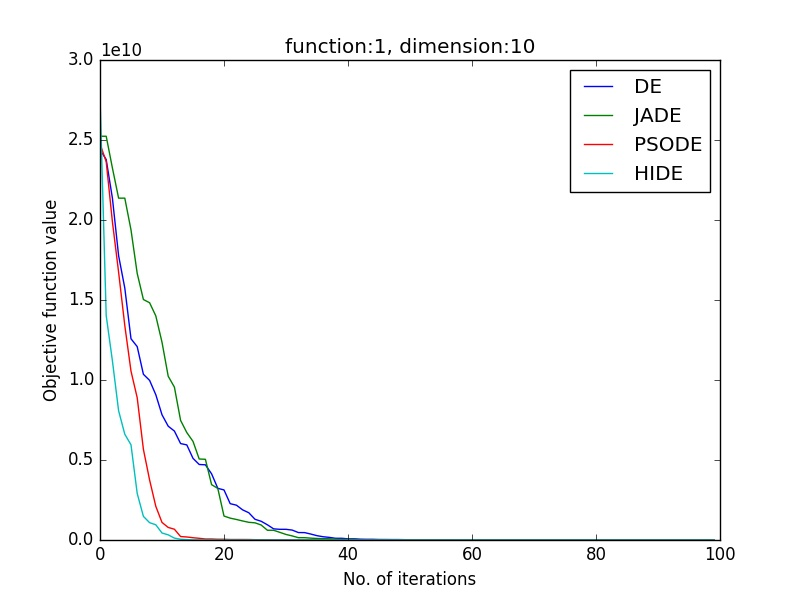
\includegraphics[width=\textwidth,natwidth=800,natheight=600]{F1D10}
        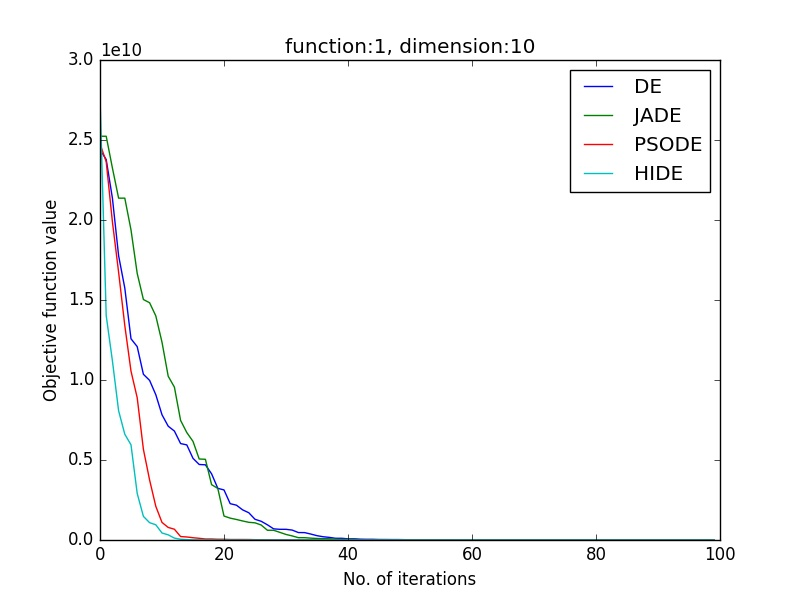
\includegraphics[width=\textwidth,natwidth=800,natheight=600]{F1D10}
        \caption{F1D10}
    \end{subfigure}
    \begin{subfigure}[b]{0.24\textwidth}
        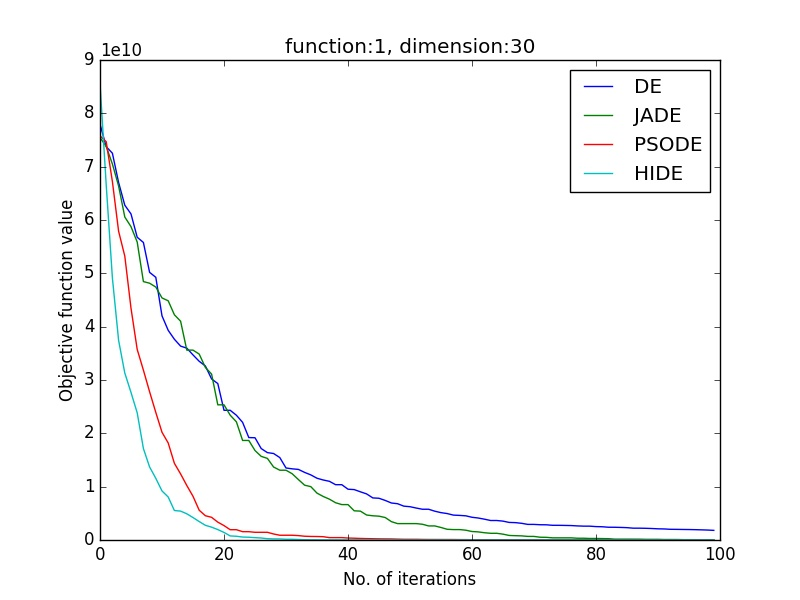
\includegraphics[width=\textwidth,natwidth=800,natheight=600]{F1D30}
        \caption{F1D30}
    \end{subfigure}    
    \begin{subfigure}[b]{0.24\textwidth}
        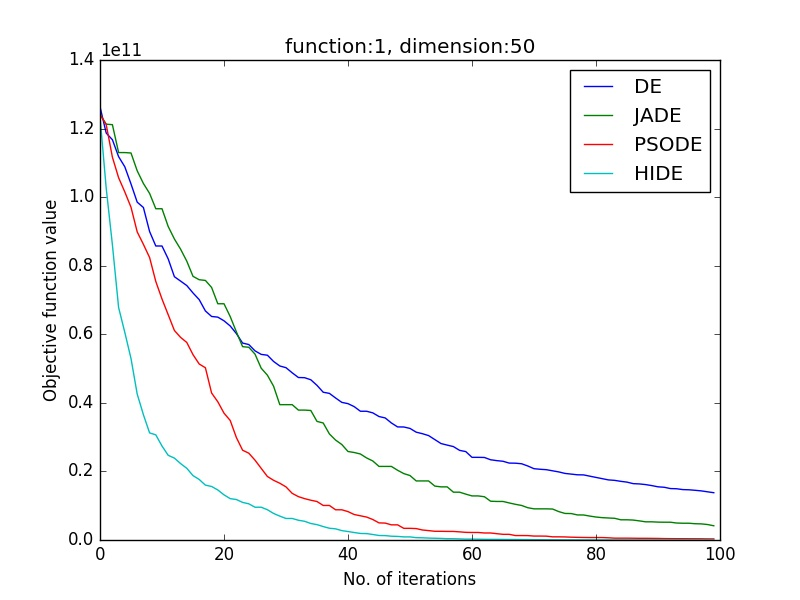
\includegraphics[width=\textwidth,natwidth=800,natheight=600]{F1D50}
        \caption{F1D10}
    \end{subfigure}
    \begin{subfigure}[b]{0.24\textwidth}
        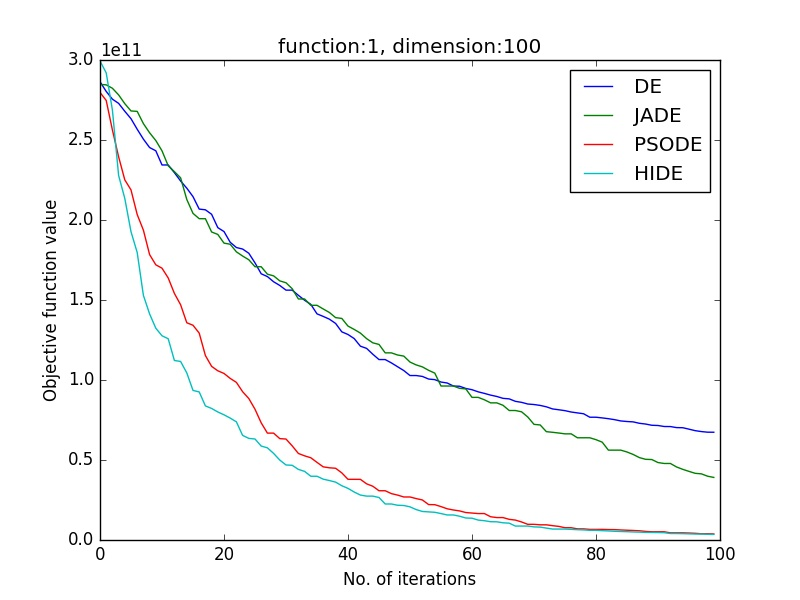
\includegraphics[width=\textwidth,natwidth=800,natheight=600]{F1D100}
        \caption{F1D30}
    \end{subfigure}

    \begin{subfigure}[b]{0.24\textwidth}
        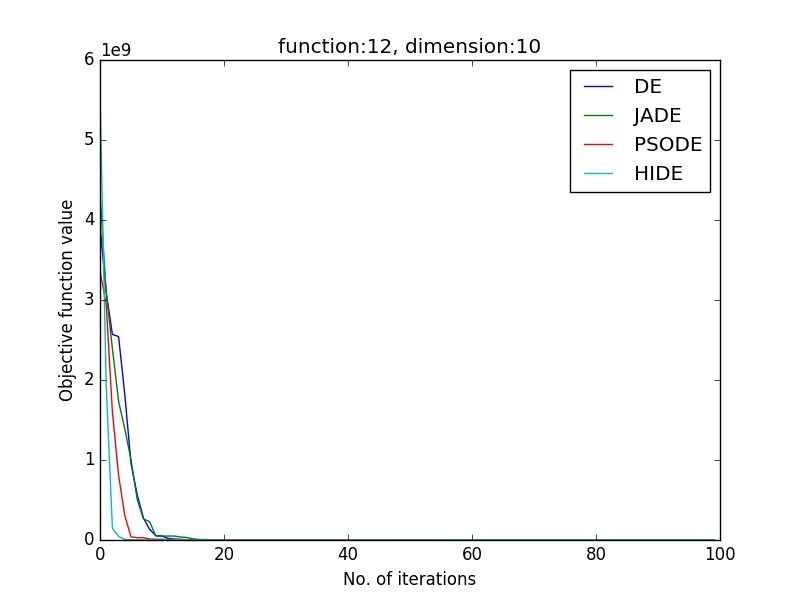
\includegraphics[width=\textwidth,natwidth=800,natheight=600]{F12D10}
        \caption{F12D10}
    \end{subfigure}
    \begin{subfigure}[b]{0.24\textwidth}
        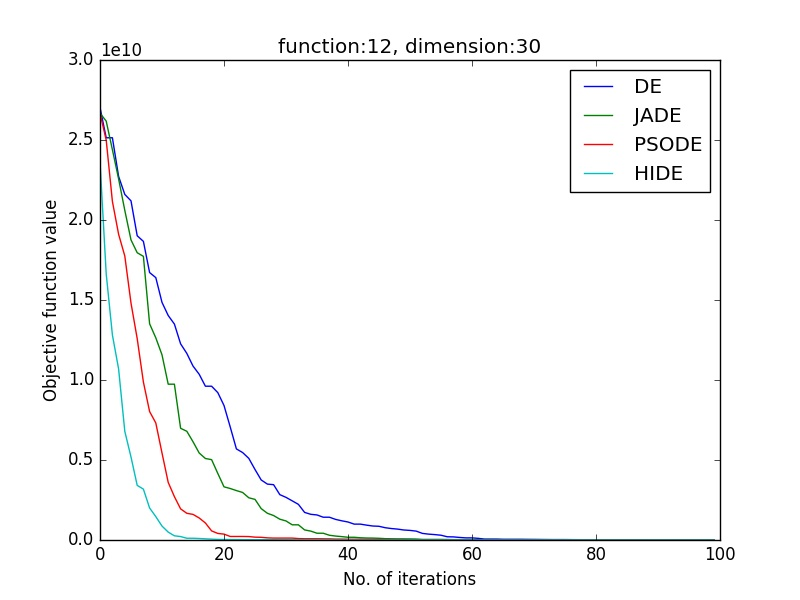
\includegraphics[width=\textwidth,natwidth=800,natheight=600]{F12D30}
        \caption{F12D30}
    \end{subfigure}        
    \begin{subfigure}[b]{0.24\textwidth}
        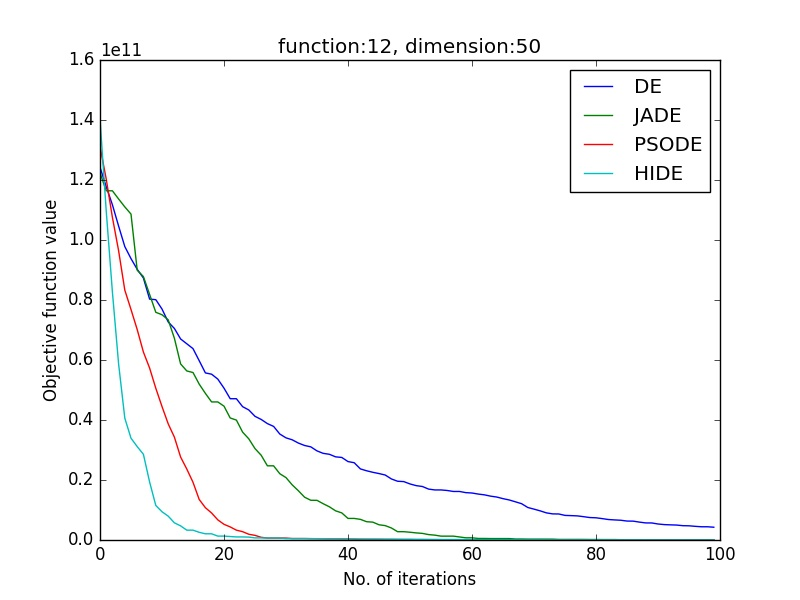
\includegraphics[width=\textwidth,natwidth=800,natheight=600]{F12D50}
        \caption{F12D50}
    \end{subfigure}
    \begin{subfigure}[b]{0.24\textwidth}
        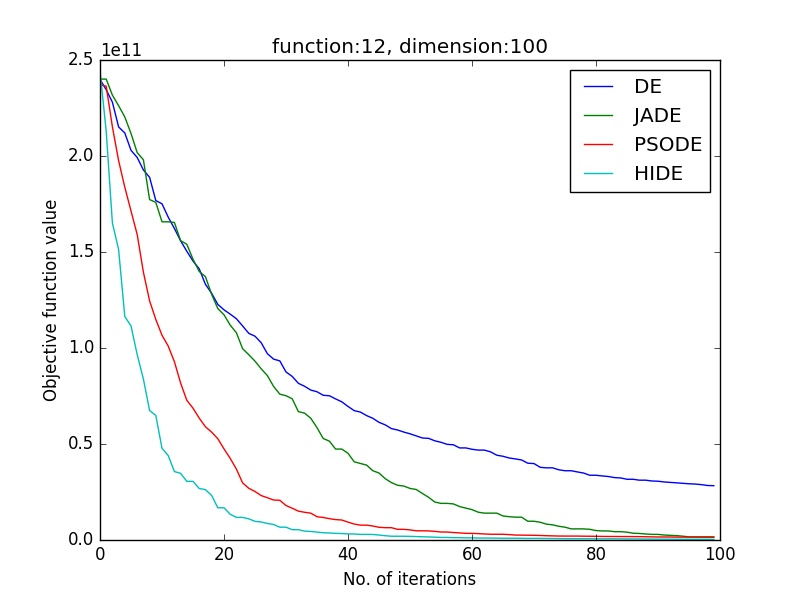
\includegraphics[width=\textwidth,natwidth=800,natheight=600]{F12D100}
        \caption{F12D100}
    \end{subfigure}

    \begin{subfigure}[b]{0.24\textwidth}
        % 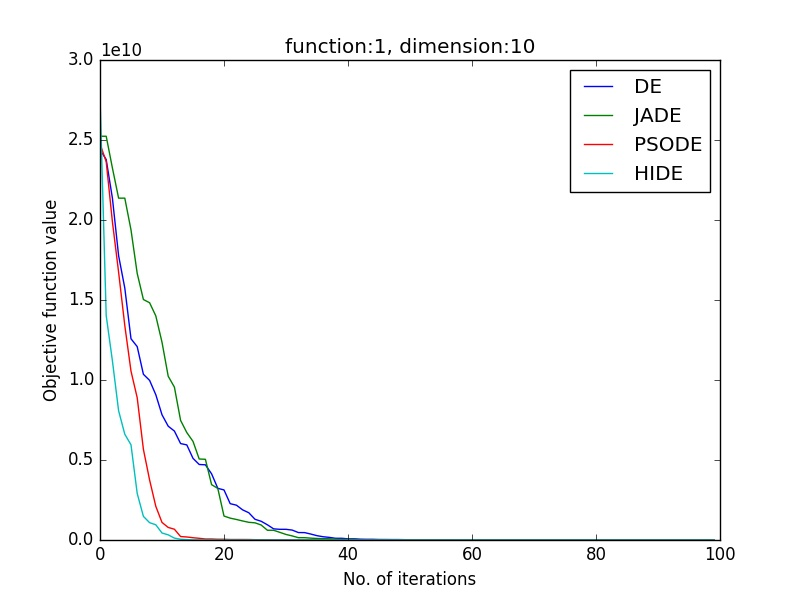
\includegraphics[width=\textwidth,natwidth=800,natheight=600]{F1D10}
        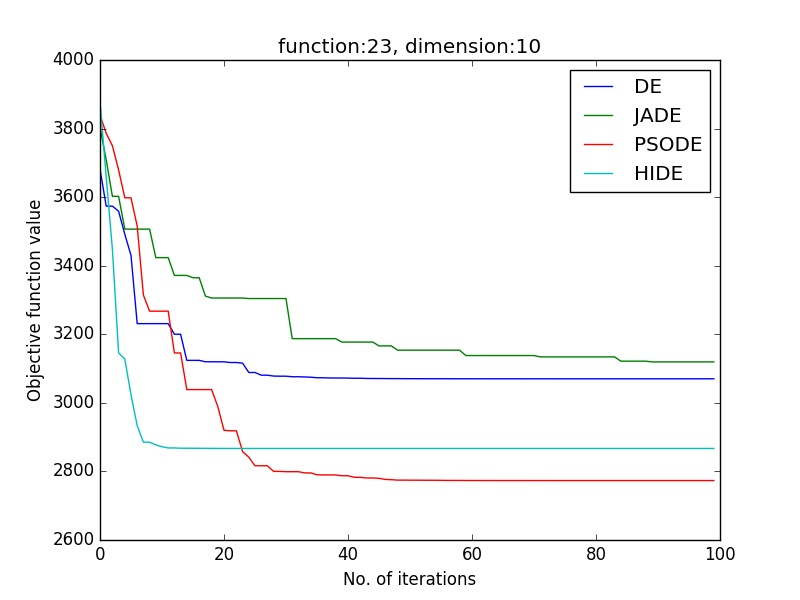
\includegraphics[width=\textwidth,natwidth=800,natheight=600]{F23D10}
        \caption{F23D10}
    \end{subfigure}
    \begin{subfigure}[b]{0.24\textwidth}
        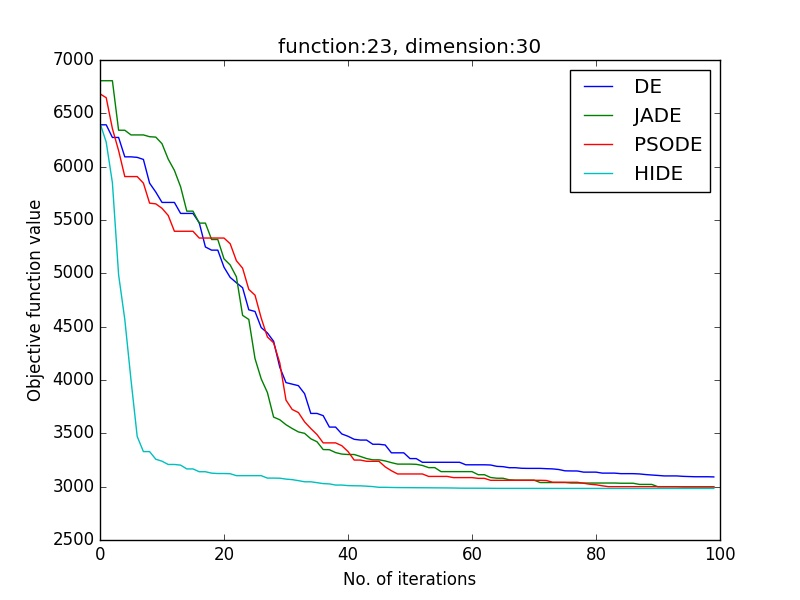
\includegraphics[width=\textwidth,natwidth=800,natheight=600]{F23D30}
        \caption{F23D30}
    \end{subfigure}    
    \begin{subfigure}[b]{0.24\textwidth}
        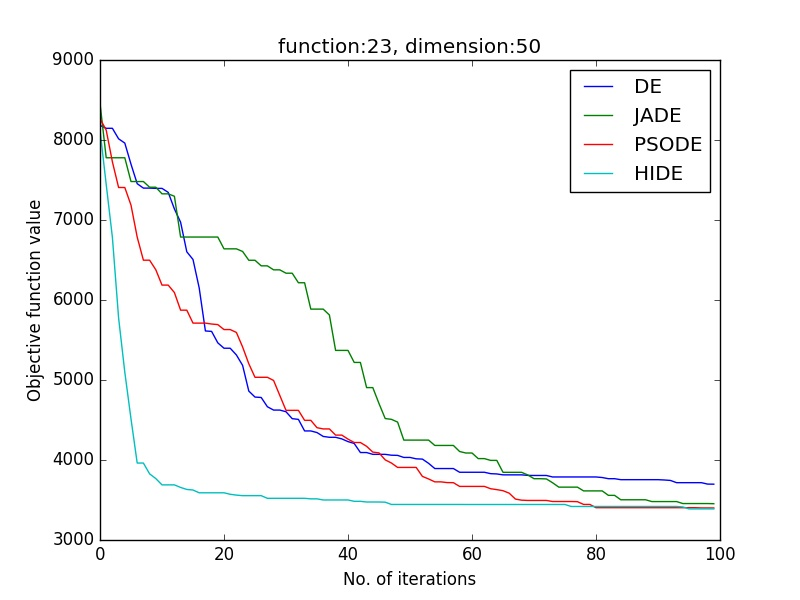
\includegraphics[width=\textwidth,natwidth=800,natheight=600]{F23D50}
        \caption{F23D50}
    \end{subfigure}
    \begin{subfigure}[b]{0.24\textwidth}
        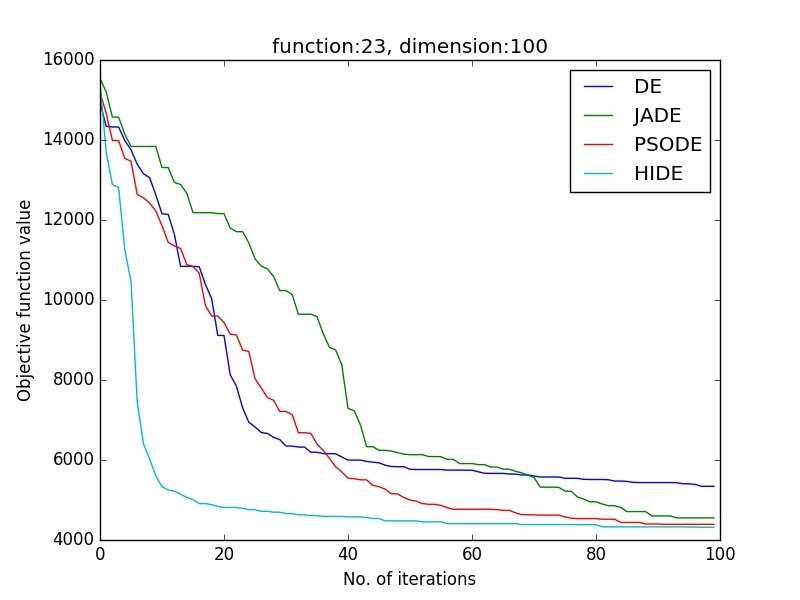
\includegraphics[width=\textwidth,natwidth=800,natheight=600]{F23D100}
        \caption{F23D100}
    \end{subfigure}

    \begin{subfigure}[b]{0.24\textwidth}
        % 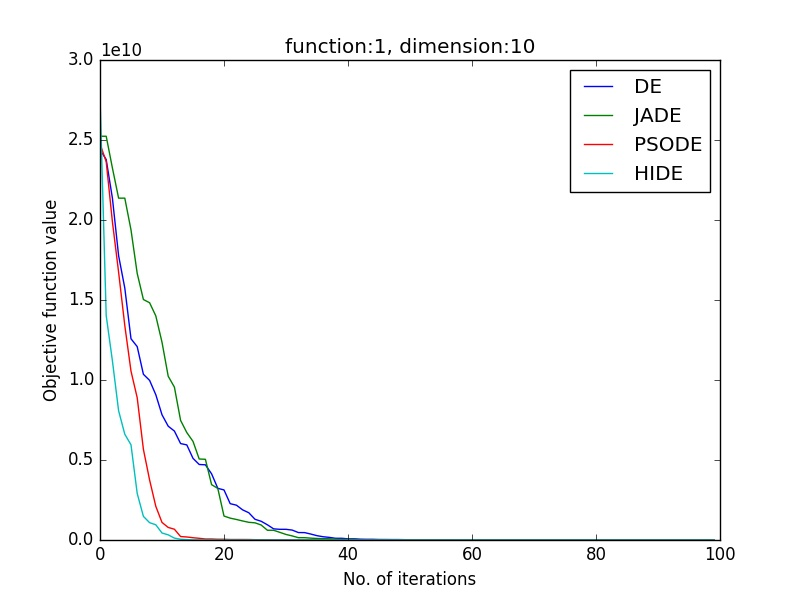
\includegraphics[width=\textwidth,natwidth=800,natheight=600]{F1D10}
        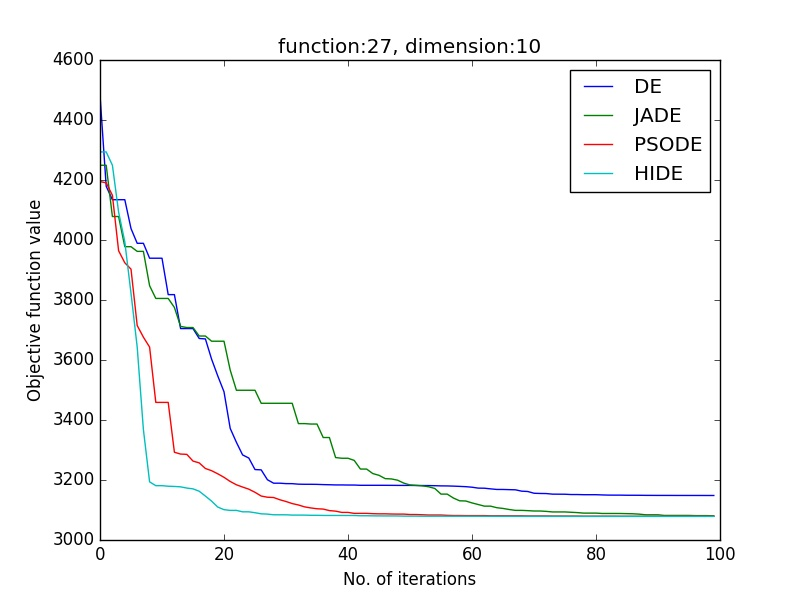
\includegraphics[width=\textwidth,natwidth=800,natheight=600]{F27D10}
        \caption{F27D10}
    \end{subfigure}
    \begin{subfigure}[b]{0.24\textwidth}
        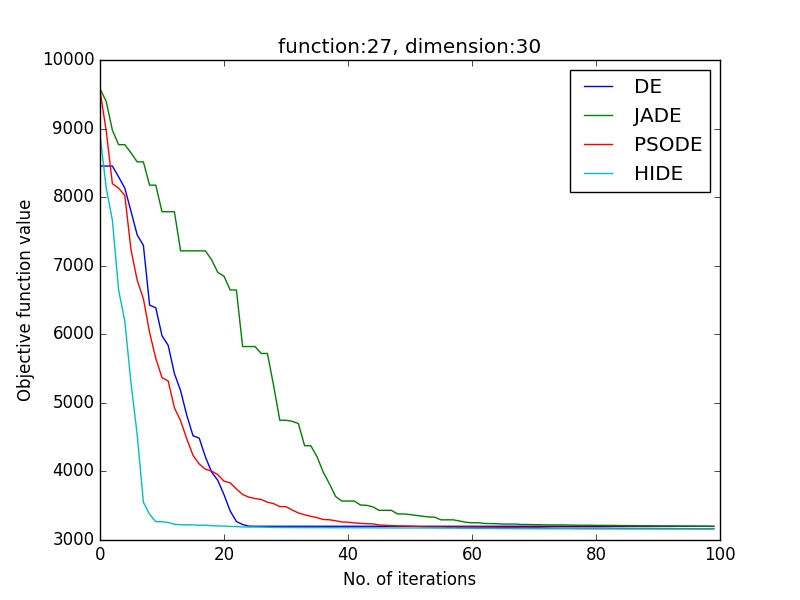
\includegraphics[width=\textwidth,natwidth=800,natheight=600]{F27D30}
        \caption{F27D30}
    \end{subfigure}    
    \begin{subfigure}[b]{0.24\textwidth}
        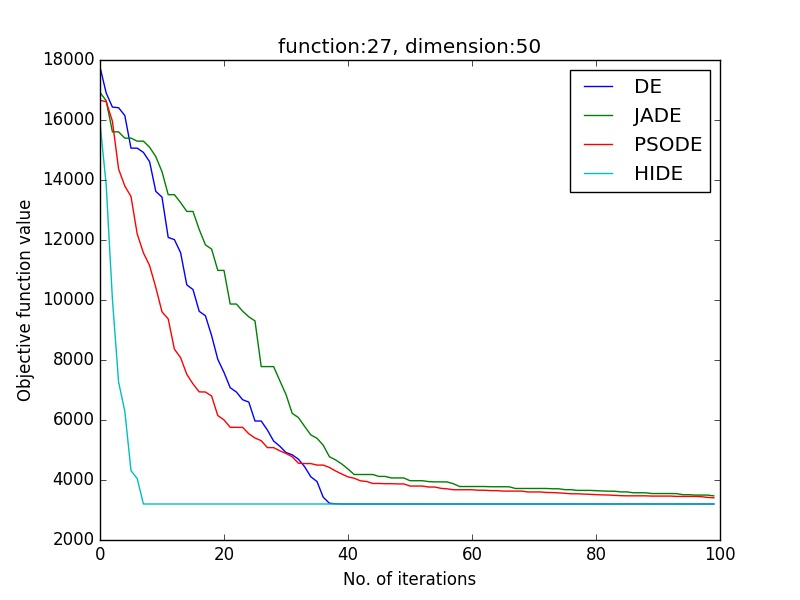
\includegraphics[width=\textwidth,natwidth=800,natheight=600]{F27D50}
        \caption{F27D50}
    \end{subfigure}
    \begin{subfigure}[b]{0.24\textwidth}
        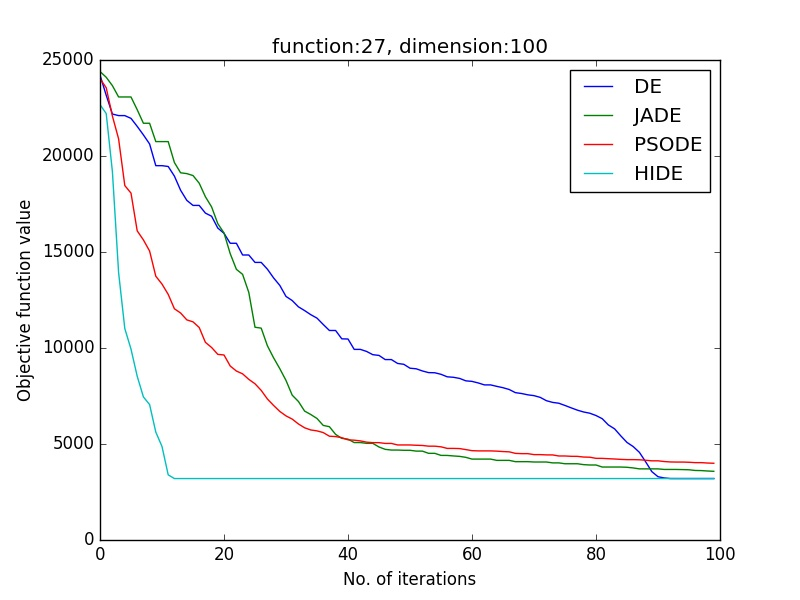
\includegraphics[width=\textwidth,natwidth=800,natheight=600]{F27D100}
        \caption{F27D100}
    \end{subfigure}

    \caption{Comparision analysis over various functions and dimensions}
    \vspace{-4mm}
\end{figure*}


\section{Conclusion}
%%summarisation of performance on different functions at all dimensions.
\begin{table}[h!]
\centering
 \begin{tabular}{|p{0.9cm}|p{1.0cm}|p{1.0cm}|p{1.0cm}}
\hline
Dim & DE & JADE & PSO-DE \\
\hline
10 & v1 & v2 & v3 \\
\hline
30 & v1 & v2 & v3 \\
\hline
50 & v1 & v2 & v3 \\
\hline
100 & v1 & v2 & v3 \\

\end{tabular}
\end{table} 
Differential Evolution is one of the most popular and widely used evolutionary meta-heuristic for the task of optimization. In this work,  we have proposed a new variant of the same called "Hierarchical Motor Differential Evolution", inspired from the hierarchical structure of the brain motor function. This approach enables the population to follow two distince motion patterns, one governed by their local leaders and one by the global leader. Based on these two influences, the individuals try to achieve the global optimum, and have shown to outperform the algorithms taken under consideration by a appreciable factor, as is clearly depicted through the numerical results and performance plots. however, since the proposed algorithm fizzles on a small fraction of the objective functions, we shall continue our quest to improve it's performance through continous modifications through our future work, and analyse it's performance on several real-world applications.~\cite{cao:frlbd} 

%\bibliographystyle{abbrv}
\bibliography{sigproc}  % sigproc.bib is the name of the Bibliography in this case


% \begin{acks}
%   The authors would like to thank Dr. Yuhua Li for providing the
%   matlab code of  the \textit{BEPS} method. 

%   The authors would also like to thank the anonymous referees for
%   their valuable comments and helpful suggestions. The work is
%   supported by the \grantsponsor{GS501100001809}{National Natural
%     Science Foundation of
%     China}{http://dx.doi.org/10.13039/501100001809} under Grant
%   No.:~\grantnum{GS501100001809}{61273304}
%   and~\grantnum[http://www.nnsf.cn/youngscientsts]{GS501100001809}{Young
%     Scientsts' Support Program}.

% \end{acks}

% \subsection{Citations}
% Citations to articles~\cite{bowman:reasoning,
% clark:pct, braams:babel, herlihy:methodology},
% conference proceedings~\cite{clark:pct} or maybe
% books \cite{Lamport:LaTeX, salas:calculus} listed
% in the Bibliography section of your
% article will occur throughout the text of your article.
% You should use BibTeX to automatically produce this bibliography;
% you simply need to insert one of several citation commands with
% a key of the item cited in the proper location in
% the \texttt{.tex} file~\cite{Lamport:LaTeX}.
% The key is a short reference you invent to uniquely
% identify each work; in this sample document, the key is
% the first author's surname and a
% word from the title.  This identifying key is included
% with each item in the \texttt{.bib} file for your article.

% The details of the construction of the \texttt{.bib} file
% are beyond the scope of this sample document, but more
% information can be found in the \textit{Author's Guide},
% and exhaustive details in the \textit{\LaTeX\ User's
% Guide}~\cite{Lamport:LaTeX}.

% This article shows only the plainest form
% of the citation command, using \texttt{{\char'134}cite}.


% \subsection{Type Changes and {\itshape Special} Characters}

% We have already seen several typeface changes in this sample.  You can
% indicate italicized words or phrases in your text with the command
% \texttt{{\char'134}textit}; emboldening with the command
% \texttt{{\char'134}textbf} and typewriter-style (for instance, for
% computer code) with \texttt{{\char'134}texttt}.  But remember, you do
% not have to indicate typestyle changes when such changes are part of
% the \textit{structural} elements of your article; for instance, the
% heading of this subsection will be in a sans serif\footnote{Another
%   footnote, here.  Let's make this a rather short one to see how it
%   looks.} typeface, but that is handled by the document class file.
% Take care with the use of\footnote{A third, and last, footnote.}  the
% curly braces in typeface changes; they mark the beginning and end of
% the text that is to be in the different typeface.

% You can use whatever symbols, accented characters, or non-English
% characters you need anywhere in your document; you can find a complete
% list of what is available in the \textit{\LaTeX\ User's Guide}
% \cite{Lamport:LaTeX}.

% \subsection{Math Equations}
% You may want to display math equations in three distinct styles:
% inline, numbered or non-numbered display.  Each of
% the three are discussed in the next sections.

% \subsubsection{Inline (In-text) Equations}
% A formula that appears in the running text is called an
% inline or in-text formula.  It is produced by the
% \textbf{math} environment, which can be
% invoked with the usual \texttt{{\char'134}begin\,\ldots{\char'134}end}
% construction or with the short form \texttt{\$\,\ldots\$}. You
% can use any of the symbols and structures,
% from $\alpha$ to $\omega$, available in
% \LaTeX~\cite{Lamport:LaTeX}; this section will simply show a
% few examples of in-text equations in context. Notice how
% this equation:
% \begin{math}
%   \lim_{n\rightarrow \infty}x=0
% \end{math},
% set here in in-line math style, looks slightly different when
% set in display style.  (See next section).

% \subsubsection{Display Equations}
% A numbered display equation---one set off by vertical space from the
% text and centered horizontally---is produced by the \textbf{equation}
% environment. An unnumbered display equation is produced by the
% \textbf{displaymath} environment.

% Again, in either environment, you can use any of the symbols
% and structures available in \LaTeX\@; this section will just
% give a couple of examples of display equations in context.
% First, consider the equation, shown as an inline equation above:
% \begin{equation}
%   \lim_{n\rightarrow \infty}x=0
% \end{equation}
% Notice how it is formatted somewhat differently in
% the \textbf{displaymath}
% environment.  Now, we'll enter an unnumbered equation:
% \begin{displaymath}
%   \sum_{i=0}^{\infty} x + 1
% \end{displaymath}
% and follow it with another numbered equation:
% \begin{equation}
%   \sum_{i=0}^{\infty}x_i=\int_{0}^{\pi+2} f
% \end{equation}
% just to demonstrate \LaTeX's able handling of numbering.


% \subsection{Tables}
% Because tables cannot be split across pages, the best
% placement for them is typically the top of the page
% nearest their initial cite.  To
% ensure this proper ``floating'' placement of tables, use the
% environment \textbf{table} to enclose the table's contents and
% the table caption.  The contents of the table itself must go
% in the \textbf{tabular} environment, to
% be aligned properly in rows and columns, with the desired
% horizontal and vertical rules.  Again, detailed instructions
% on \textbf{tabular} material
% are found in the \textit{\LaTeX\ User's Guide}.

% Immediately following this sentence is the point at which
% Table~\ref{tab:freq} is included in the input file; compare the
% placement of the table here with the table in the printed
% output of this document.

% \begin{table}
%   \caption{Frequency of Special Characters}
%   \label{tab:freq}
%   \begin{tabular}{ccl}
%     \toprule
%     Non-English or Math&Frequency&Comments\\
%     \midrule
%     \O & 1 in 1,000& For Swedish names\\
%     $\pi$ & 1 in 5& Common in math\\
%     \$ & 4 in 5 & Used in business\\
%     $\Psi^2_1$ & 1 in 40,000& Unexplained usage\\
%   \bottomrule
% \end{tabular}
% \end{table}

% To set a wider table, which takes up the whole width of the page's
% live area, use the environment \textbf{table*} to enclose the table's
% contents and the table caption.  As with a single-column table, this
% wide table will ``float'' to a location deemed more desirable.
% Immediately following this sentence is the point at which
% Table~\ref{tab:commands} is included in the input file; again, it is
% instructive to compare the placement of the table here with the table
% in the printed output of this document.


% \begin{table*}
%   \caption{Some Typical Commands}
%   \label{tab:commands}
%   \begin{tabular}{ccl}
%     \toprule
%     Command &A Number & Comments\\
%     \midrule
%     \texttt{{\char'134}author} & 100& Author \\
%     \texttt{{\char'134}table}& 300 & For tables\\
%     \texttt{{\char'134}table*}& 400& For wider tables\\
%     \bottomrule
%   \end{tabular}
% \end{table*}
% % end the environment with {table*}, NOTE not {table}!

% It is strongly recommended to use the package booktabs~\cite{Fear05}
% and follow its main principles of typography with respect to tables:
% \begin{enumerate}
% \item Never, ever use vertical rules.
% \item Never use double rules.
% \end{enumerate}
% It is also a good idea not to overuse horizontal rules.


% \subsection{Figures}

% Like tables, figures cannot be split across pages; the best placement
% for them is typically the top or the bottom of the page nearest their
% initial cite.  To ensure this proper ``floating'' placement of
% figures, use the environment \textbf{figure} to enclose the figure and
% its caption.

% This sample document contains examples of \texttt{.eps} files to be
% displayable with \LaTeX.  If you work with pdf\LaTeX, use files in the
% \texttt{.pdf} format.  Note that most modern \TeX\ systems will convert
% \texttt{.eps} to \texttt{.pdf} for you on the fly.  More details on
% each of these are found in the \textit{Author's Guide}.

% \begin{figure}
% 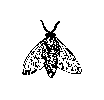
\includegraphics{fly}
% \caption{A sample black and white graphic.}
% \end{figure}

% \begin{figure}
% 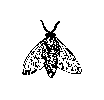
\includegraphics[height=1in, width=1in]{fly}
% \caption{A sample black and white graphic
% that has been resized with the \texttt{includegraphics} command.}
% \end{figure}


% As was the case with tables, you may want a figure that spans two
% columns.  To do this, and still to ensure proper ``floating''
% placement of tables, use the environment \textbf{figure*} to enclose
% the figure and its caption.  And don't forget to end the environment
% with \textbf{figure*}, not \textbf{figure}!

% \begin{figure*}
% 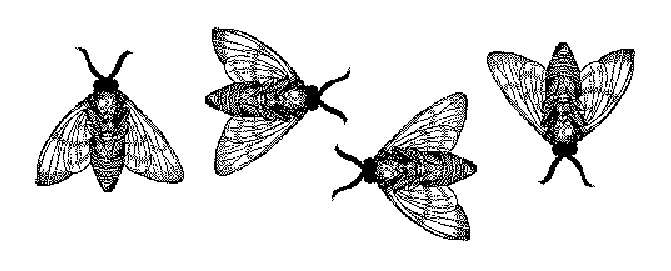
\includegraphics{flies}
% \caption{A sample black and white graphic
% that needs to span two columns of text.}
% \end{figure*}


% \begin{figure}
% 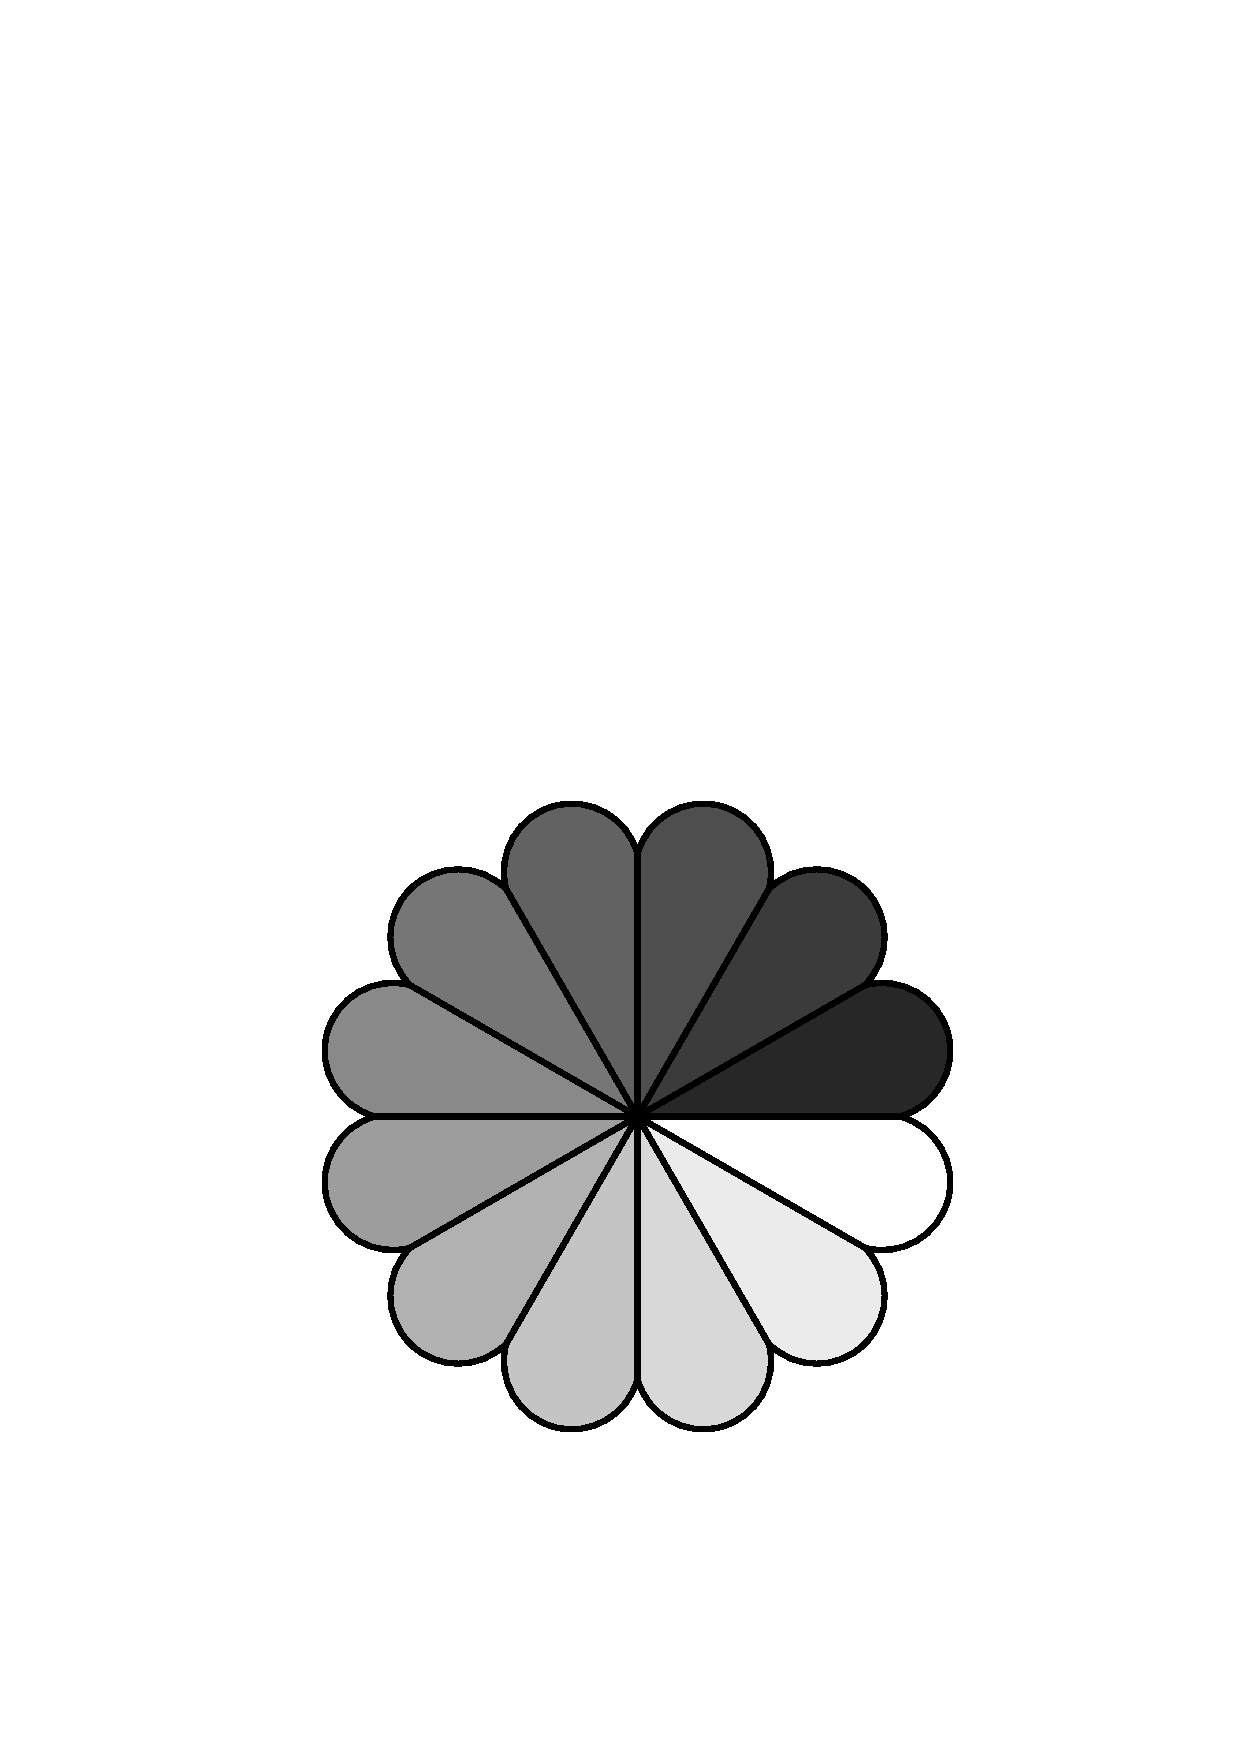
\includegraphics[height=1in, width=1in]{rosette}
% \caption{A sample black and white graphic that has
% been resized with the \texttt{includegraphics} command.}
% \end{figure}

% \subsection{Theorem-like Constructs}

% Other common constructs that may occur in your article are the forms
% for logical constructs like theorems, axioms, corollaries and proofs.
% ACM uses two types of these constructs:  theorem-like and
% definition-like.

% Here is a theorem:
% \begin{theorem}
%   Let $f$ be continuous on $[a,b]$.  If $G$ is
%   an antiderivative for $f$ on $[a,b]$, then
%   \begin{displaymath}
%     \int^b_af(t)\,dt = G(b) - G(a).
%   \end{displaymath}
% \end{theorem}

% Here is a definition:
% \begin{definition}
%   If $z$ is irrational, then by $e^z$ we mean the
%   unique number that has
%   logarithm $z$:
%   \begin{displaymath}
%     \log e^z = z.
%   \end{displaymath}
% \end{definition}

% The pre-defined theorem-like constructs are \textbf{theorem},
% \textbf{conjecture}, \textbf{proposition}, \textbf{lemma} and
% \textbf{corollary}.  The pre-defined de\-fi\-ni\-ti\-on-like constructs are
% \textbf{example} and \textbf{definition}.  You can add your own
% constructs using the \textsl{amsthm} interface~\cite{Amsthm15}.  The
% styles used in the \verb|\theoremstyle| command are \textbf{acmplain}
% and \textbf{acmdefinition}.

% Another construct is \textbf{proof}, for example,

% \begin{proof}
%   Suppose on the contrary there exists a real number $L$ such that
%   \begin{displaymath}
%     \lim_{x\rightarrow\infty} \frac{f(x)}{g(x)} = L.
%   \end{displaymath}
%   Then
%   \begin{displaymath}
%     l=\lim_{x\rightarrow c} f(x)
%     = \lim_{x\rightarrow c}
%     \left[ g{x} \cdot \frac{f(x)}{g(x)} \right ]
%     = \lim_{x\rightarrow c} g(x) \cdot \lim_{x\rightarrow c}
%     \frac{f(x)}{g(x)} = 0\cdot L = 0,
%   \end{displaymath}
%   which contradicts our assumption that $l\neq 0$.
% \end{proof}

% \section{Conclusions}
% This paragraph will end the body of this sample document.
% Remember that you might still have Acknowledgments or
% Appendices; brief samples of these
% follow.  There is still the Bibliography to deal with; and
% we will make a disclaimer about that here: with the exception
% of the reference to the \LaTeX\ book, the citations in
% this paper are to articles which have nothing to
% do with the present subject and are used as
% examples only.
% %\end{document}  % This is where a 'short' article might terminate



% \appendix
% %Appendix A
% \section{Headings in Appendices}
% The rules about hierarchical headings discussed above for
% the body of the article are different in the appendices.
% In the \textbf{appendix} environment, the command
% \textbf{section} is used to
% indicate the start of each Appendix, with alphabetic order
% designation (i.e., the first is A, the second B, etc.) and
% a title (if you include one).  So, if you need
% hierarchical structure
% \textit{within} an Appendix, start with \textbf{subsection} as the
% highest level. Here is an outline of the body of this
% document in Appendix-appropriate form:
% \subsection{Introduction}
% \subsection{The Body of the Paper}
% \subsubsection{Type Changes and  Special Characters}
% \subsubsection{Math Equations}
% \paragraph{Inline (In-text) Equations}
% \paragraph{Display Equations}
% \subsubsection{Citations}
% \subsubsection{Tables}
% \subsubsection{Figures}
% \subsubsection{Theorem-like Constructs}
% \subsubsection*{A Caveat for the \TeX\ Expert}
% \subsection{Conclusions}
% \subsection{References}
% Generated by bibtex from your \texttt{.bib} file.  Run latex,
% then bibtex, then latex twice (to resolve references)
% to create the \texttt{.bbl} file.  Insert that \texttt{.bbl}
% file into the \texttt{.tex} source file and comment out
% the command \texttt{{\char'134}thebibliography}.
% % This next section command marks the start of
% % Appendix B, and does not continue the present hierarchy
% \section{More Help for the Hardy}

% Of course, reading the source code is always useful.  The file
% \path{acmart.pdf} contains both the user guide and the commented
% code.


